\documentclass[a4paper,11pt,twoside,openright]{article}

\usepackage[toc,page]{appendix}
\usepackage{amsmath}
\usepackage{geometry}
\usepackage{graphicx}
\usepackage{subcaption}
\usepackage{multirow}
\usepackage[section]{placeins}
\usepackage{array}
\usepackage[nottoc,numbib]{tocbibind}
\usepackage{multicol}
\usepackage{wrapfig}
%\usepackage{titlesec}

\geometry{margin=1in}
\graphicspath{ {Images/} }

\newcolumntype{?}[1]{!{\vrule width #1}}
\newcommand{\Mod}[1]{\ (\mathrm{mod}\ #1)}

\let\oldsection\section
\def\section{\cleardoublepage\oldsection}

%\setcounter{tocdepth}{4}

%\titleformat{\paragraph}
%{\normalfont\normalsize\bfseries}{\theparagraph}{1em}{}
%\titlespacing*{\paragraph}
%{0pt}{3.25ex plus 1ex minus .2ex}{1.5ex plus .2ex}

\begin{document}

%%%%%%%%%%%%%%%%%%%%%%%%%%%%%%%%%%%%%%%%%%%%%%%%%%%%%%%%%%%%%%%%%%%%%%%%%%%%%%%
% TITLEPAGE                                                                   %
%%%%%%%%%%%%%%%%%%%%%%%%%%%%%%%%%%%%%%%%%%%%%%%%%%%%%%%%%%%%%%%%%%%%%%%%%%%%%%%
\pagenumbering{gobble}
\centering
\vspace*{6cm}
        {\huge Developing AntBot: \par A navigational system inspired by \par the
          insect brain \par}
\vspace{1cm}
{\Large \textit{Robert E. F. Mitchell}}

\vspace{3cm}

{\large Master of Informatics \par}
{\large Informatics \par}
{\large School of Informatics \par}
{\large The University of Edinburgh \par}
\large \today \par

\vfill
Supervised by\par
Dr. Barbara Webb

\newpage
\thispagestyle{empty}
\mbox{}
\newpage

%%%%%%%%%%%%%%%%%%%%%%%%%%%%%%%%%%%%%%%%%%%%%%%%%%%%%%%%%%%%%%%%%%%%%%%%%%%%%%%
% ACKNOWLEDGEMENTS                                                            %
%%%%%%%%%%%%%%%%%%%%%%%%%%%%%%%%%%%%%%%%%%%%%%%%%%%%%%%%%%%%%%%%%%%%%%%%%%%%%%%
\pagenumbering{roman}
\centering
{\LARGE \textbf{Acknowledgements}}
\begin{flushleft}
  {\small I would like to thank the following people, each of whom as
    provided support, academic or otherwise throughout this work.

    \begin{itemize}
    \item{Prof. Barbara Webb - Thank you for your guidance and insight
      throughout the project. The support and constant feedback you
      have provided in your role as supervisor have been invaluable.}

    \item{The insect robotics group - I would also like to thank the
      wider insect robotics group, all of whom have been approachable
      and open to discussion throughout. In particular, I would like
      to thank Jan Stankiewicz. Our conversations regarding the
      operation of the Central Complex and biological approaches to
      optical flow sensitivity in insects greatly aided my
      understanding of the topics and helped me develop much of the
      work in this paper. }

    \item{My parents: Tom, and Linda Mitchell - Your unwavering
      support throughout my education, of my subject
      choices, and of my goals of further study have allowed and
      encouraged to push beyond my limits and work to the best of my
      ability. I can never thank you enough.
        }

    \item{My closest friends: Marko Kerr, Ethan Piddington, and Nik
      Hogarth - Regardless of how busy or detached I have been through
      this past year, I have always known I could step back into the
      circle as if no time had passed at all. Thank you for being
      there. }

    \item{John ``Hedge'' Hall - It is fair you to say that you have
      been somewhat of a mentor figure throughout my University
      career. In the last two years, our conversations on academia,
      success, education, and whatever philosophy you happened to be
      reading about at the time, have helped me maintain a healthy
      perspective on life. You introduced me to the practice of
      meditation, which has helped me maintain a cool head, where
      previously I would be absorbed by stress. Thank you for giving
      me a more robust approach to mental health, and for showing me
      that getting older does not mean growing up.}

    \item{Alana L. White - Your enduring support and love throughout
      these last years has kept me grounded in an otherwise turbulent
      time. You were always there for me when I needed you most but
      best of all, you were there for me when I did not. You were the
      constant on which I could always rely. Thank you, for everything.}
    \end{itemize}
  }
\end{flushleft}

\newpage
\thispagestyle{empty}
\mbox{}
\newpage

%%%%%%%%%%%%%%%%%%%%%%%%%%%%%%%%%%%%%%%%%%%%%%%%%%%%%%%%%%%%%%%%%%%%%%%%%%%%%%%
% DECLARATION                                                                 %
%%%%%%%%%%%%%%%%%%%%%%%%%%%%%%%%%%%%%%%%%%%%%%%%%%%%%%%%%%%%%%%%%%%%%%%%%%%%%%%
\centering
{\LARGE\textbf{Declaration}}
\begin{flushleft}
  {\small
    I declare that this dissertation was composed by myself, the work
    contained herein is my own except where explicitly stated otherwise
    in the text, and that this work has not been submitted for any other
    degree or professional qualification except as specified.
    \par

    \textit{Robert Mitchell}}

\end{flushleft}

\newpage
\thispagestyle{empty}
\mbox{}
\newpage

%%%%%%%%%%%%%%%%%%%%%%%%%%%%%%%%%%%%%%%%%%%%%%%%%%%%%%%%%%%%%%%%%%%%%%%%%%%%%%%
% ABSTRACT                                                                    %
%%%%%%%%%%%%%%%%%%%%%%%%%%%%%%%%%%%%%%%%%%%%%%%%%%%%%%%%%%%%%%%%%%%%%%%%%%%%%%%
\centering
{\LARGE\textbf{Abstract}}
\begin{flushleft}
  {\small Ants are incredible navigators. With limited sensory and
    computational capabilities they are able to perform robust
    navigation over relatively vast distances, through varying
    terrains and lighting conditions. How this is done is not quite
    known, however models for individual aspects of the navigational
    process have been constructed and demonstrated in recent years in
    simulation, and on robot platforms.  We take two such models, the
    Mushroom Body circuit for Visual Navigation and the Central
    Complex model for Path Integration. We combine these with a
    biologically plausible neural model for collision avoidance to
    provide a conceptually complete \textit{base model} for insect
    navigation, the Extended Central Complex. This model has been
    implemented on a robot platform, AntBot. In an effort to develop
    the model we also present several advancements to the AntBot
    platform, experimentation with an alternative optical flow method
    for collision avoidance, experiments with the Central Complex
    model to address some isssues with previous tests, and promising
    (though informal) early results indicating the plausibility of our
    approach. Finally, we present suggestions for future work on both
    the component models and our combined model, as well as
    recommendations for future development of the AntBot platform.}
\end{flushleft}
\newpage

%%%%%%%%%%%%%%%%%%%%%%%%%%%%%%%%%%%%%%%%%%%%%%%%%%%%%%%%%%%%%%%%%%%%%%%%%%%%%%%
% CONTENTS                                                                    %
%%%%%%%%%%%%%%%%%%%%%%%%%%%%%%%%%%%%%%%%%%%%%%%%%%%%%%%%%%%%%%%%%%%%%%%%%%%%%%%
\tableofcontents
\newpage

%%%%%%%%%%%%%%%%%%%%%%%%%%%%%%%%%%%%%%%%%%%%%%%%%%%%%%%%%%%%%%%%%%%%%%%%%%%%%%%
% FIGURES                                                                     %
%%%%%%%%%%%%%%%%%%%%%%%%%%%%%%%%%%%%%%%%%%%%%%%%%%%%%%%%%%%%%%%%%%%%%%%%%%%%%%%
\listoffigures
\newpage

%%%%%%%%%%%%%%%%%%%%%%%%%%%%%%%%%%%%%%%%%%%%%%%%%%%%%%%%%%%%%%%%%%%%%%%%%%%%%%%
% TABLES                                                                      %
%%%%%%%%%%%%%%%%%%%%%%%%%%%%%%%%%%%%%%%%%%%%%%%%%%%%%%%%%%%%%%%%%%%%%%%%%%%%%%%
\listoftables
\newpage
\thispagestyle{empty}
\mbox{}
\newpage

%%%%%%%%%%%%%%%%%%%%%%%%%%%%%%%%%%%%%%%%%%%%%%%%%%%%%%%%%%%%%%%%%%%%%%%%%%%%%%%
% INTRODUCTION                                                                %
%%%%%%%%%%%%%%%%%%%%%%%%%%%%%%%%%%%%%%%%%%%%%%%%%%%%%%%%%%%%%%%%%%%%%%%%%%%%%%%
\pagenumbering{arabic}

\raggedright

\section{ Introduction }
Navigation is a complex task. Determining a sequence of actions to reach a
known location based on a combination of sensory inputs requires a lot of
computational power. Desert ants are capable of performing such a task
over comparitively vast distances with limited, low resolution sensory
information and remarkable efficiency. While the exact method by which
the ants perform this task is still unknown, a reasonably complete navigational
model can be constructed from existing physiologically plausible components,
which may mimic the insect behaviour.
\newline
\par

In this paper we introduce a theoretical combined model, the Extended
Central Complex (ECX) model for insect navigation. To be clear, there
is no (known) physiological basis for such a model; however, it is
biologically feasible and may provide insight into the operation of
the real insect brain. The ECX model combines the tasks of Visual
Navigation, Path Integration, and Collision Avoidance; using the
Mushroom Body Circuit (MB) \cite{Ardin2016}, the Central Complex model
(CX) \cite{Stone2017}, and Optical Flow Collision Avoidance (OFCA)
\cite{Mitchell2018, Stewart2010} for each task at a low level, then
combining their outputs to get a form of higher navigational
processing (similar to the weighted ``base model'' described in
\cite{Webb2019}).  The ECX model is a modified Central Complex model,
named simply to ensure distinction between the two models. The
individual components are all biologically plausible and two of three
(the MB and CX) are known to have a physiological
basis. \cite{Ardin2016, Stone2017, Mitchell2018, Stewart2010,
  Julien2017}.
\newline
\par

This project primarily extends the work done in
\cite{Mitchell2018}. Therefore we continue using the AntBot platform; a
robot constructed for the express purpose of experimenting with the
algorithms in the \textit{Ant Navigational Toolkit}
\cite{Eberding2016, Wehner2009}.

\subsection{ Motivation }
Currently, a full base model for insect navigation does not exist
\cite{Webb2019}. We here aim to take the abstraction presented by
\textit{Webb} and create a biologically plausible implementation using
our three-system approach. Both the MB and CX models have been
implemented and tested on AntBot previously \cite{Scimeca2017,
  Mitchell2018, Eberding2016, Zhang2017}, and a model combining the
two has also been constructed by \textit{Zhang} \cite{Zhang2017}.
This combined model is used as a basis for our own and will be
discussed further in Section \ref{CXMBBackground}.
\newline
\par

The previous AntBot implementations have demonstrated good performance
of the CX and MB models individually \cite{Scimeca2017,
  Mitchell2018}. Performance of a combined system has also been shown
to be reasonable, however, it is less consistent than we would desire
\cite{Zhang2017}. In the combined model tests from \cite{Zhang2017} we
note two key methodological problems: a fixed outbound route, and
fixed component weightings; the fixed outbound route was also present
in the CX experiments conducted by \textit{Scimeca}. We address the
former by adding the OFCA component to our model; as in
\cite{Mitchell2018}, the AntBot will follow a non-deterministic
outbound route through an arena with obejcts present. The latter
brings up the more complicated question of plausible synaptic
plasticity which, though undoubtedly interesting, lies outside the
scope of this project (though we will discuss the concept to a limited
extent). It is worth noting that there may also have been unknown
tecnical issues with the robot which affected the results of
\cite{Zhang2017}, making them less consistent than they should be in
reality (see \cite{Mitchell2018} and later in this work).
\newline
\par

While \cite{Mitchell2018} provides a reasonable collision avoidance
system based on optical flow, it does not fit so neatly into the ECX
model.Therefore we aim to explore an alternative yet still
biologically plausible collision avoidance system which will fit into
the ECX model.
\newline
\par

Our ultimate goal is to provide some insight into the precise biological
systems in play during a point-to-point navigational task.

\subsection { Practical Goals }
The original aim of this project was to build on the experimental
scenario from \cite{Mitchell2018}. The robot would be tested by
allowing it to navigate through a cluttered environment using a
collision avoidance system. The navigational systems would then be
tasked with bringing the robot home through the same cluttered
environment using a combination of visual information, a path
integration vector, and collision avoidance.
\newline
\par

In order to achieve this experimental goal, the project was broken down
into four stages:

\begin{enumerate}
\item{The first stage involved solving some choice technical issues
  picked up by \cite{Mitchell2018}; making any hardware/software adjustments
  required to provide a solid foundation on which to develop.}

\item{We then began investigating existing systems. This stage will
  involved research and review of new topics (the main one being the
  Central Complex model for Path Integration), and their
  implementations on the robot (if present). This stage also looked to
  test the CX model in a non-deterministic navigational task (see
  Section \ref{sec:methods}).}

\item{This stage  involved the set up and testing of the individual components
  of the ECX model. Building the modified optical flow system, using the work
  from \textit{Zhang} to combine the MB model with the CX, and finally, putting
  the three pieces together to form a complete implementation.}

\item{Finally, the collection and compilation of results from the combined system
and the individual systems.}
\end{enumerate}

\subsection { Results }
This work is based on work done previously by Leonard Eberding, Luca Scimeca,
Zhaoyu Zhang, and Robert Mitchell.
\cite{Eberding2016, Scimeca2017, Zhang2017, Mitchell2018}.
\newline

The significant contributions of this project are:
\begin{enumerate}
\item{
  Research and installation of a new compass sensor for the AntBot control
  systems.
}

\item{
  Refactoring a sizable amount of code to make AntBot more usable for this
  project, and make it more accessible for future students.
}

\item{
  Addition of a calibration system to allow the user to auto-detect the position
  of the camera lens attachment (see Section \ref{sec:mod}).
}

\item{
  Results gathered for the Central Complex model using a non-deterministic
  outbound route.
}

\item{
  Construction of a video recording tool to allow processed
  image frames to be recorded from the robot for later viewing and
  offline analysis.
}

\item{ Construction of new, larger, more robust tussocks for use in
  experimentation (as realistic obstacles and visual landmarks), based
  on the recommendation in \cite{Mitchell2018}}

\item{ Results definitively showing the impracticality of a focus of
    expansion based system for collision avoidance and justifying
    continued use of matched filters.
}

\item{ Identification and correction of a bug in the visual preprocessing system
  to raise the framerate from 2fps to approximately 10fps under normal usage.}

\item{ Construction of a neural collision avoidance model based on the
  matched filter system from \cite{Mitchell2018, Stewart2010}. }


\item{
  Implementation of a biologically plausible ``base model'' for
  insect navigation, the Extended Central Complex (ECX) model.
}

\item{ Collection of evidence to support the recommendation that the
  current AntBot platform be retired, and suggestions for a new
  platform based on lessons learned from the AntBot.  }

\end{enumerate}
\newpage

%%%%%%%%%%%%%%%%%%%%%%%%%%%%%%%%%%%%%%%%%%%%%%%%%%%%%%%%%%%%%%%%%%%%%%%%%%%%%%%
% BACKGROUND                                                                  %
%%%%%%%%%%%%%%%%%%%%%%%%%%%%%%%%%%%%%%%%%%%%%%%%%%%%%%%%%%%%%%%%%%%%%%%%%%%%%%%
% Brief summaries of OF and MB, more detailed discussion of CX
\section{ Background }
This project builds directly upon \cite{Mitchell2018}. We first provide a review
of the relevant background topics from that paper, before developing the key
ideas further for this project. This will be a very brief summary of the work
that took place and any relevant results or new perspectives.


\subsection{ The Focus of Expansion for Collision Avoidance } \label{OFBackground}
Optical flow is the 2D approximation of image flow, the 3D motion
observed in a scene over consecutive image frames. Optical flow is
described by a field of vectors (a \textit{flow field}) which show how
tracked points move between frames. It is a large and
diverse area of study.  Consequently, we will not provide a complete
background on the fundamental principles. We will give only a succinct
background of the concepts necessary for this paper. A comprehensive
introduction to the topic is given by \textit{O'Donovan} in
\cite{ODonovan2005}.
\newline
\par

The main driving point in this paper is the integration of multiple
navigational systems into a single model, namely, the Central Complex.
Optical flow filtering worked well for a standalone collision
avoidance system \cite{Stewart2010, Mitchell2018}, however it does not
fit so intuitively into the CX model. We therefore investigate an
alternate approach. The relevant background revisits the concept of
the \textit{focus of expansion} (FOE) from \cite{Mitchell2018,
  ODonovan2005}.  The FOE is defined as the point from which all
optical flow vectors originate. The location of the FOE, and its
relationship with the rest of the flow field, can give us information
about a 3D scene from a 2D image (e.g. image depth)\cite{ODonovan2005,
  Souhila2007}.
\newline
\par

In \cite{Mitchell2018}, the FOE was used only to compute
time-to-contact with an obstacle. In this work, we instead attempt to
use it directly to determine the potential location of an
obstacle. Following \cite{Mitchell2018} we will be using a dense optic
flow field (tracking motion for every pixel in the image) as the
computation of sparse fields was shown to be unreliable on the
AntBot. This potentially makes the problem more difficult; the basic
method for calculating the FOE given by \cite{ODonovan2005} is
computationally complex for a dense flow field
\cite{Mitchell2018}. The time taken to compute may become
prohibitive. A common, reliable and intuitive method of computing the
FOE is the Least Squared-Error (LSE) method \cite{Tistarelli1991,
  ODonovan2005, Vanderstap2012}. This method also appears to be in use
in \cite{Souhila2007}, a major inspiration for the optical flow
methods presented in \cite{Mitchell2018}.

\subsubsection{The Least Squared-Error method}
This is the method given by \textit{O'Donovan} and discussed in
\cite{Mitchell2018}. The FOE is computed simply as:

\begin{equation}
  \label{eq:foe}
  FOE = (A^TA)^{-1}A^T\mathbf{b}
\end{equation}

\begin{equation*}
  \begin{split}
 A =
\begin{bmatrix}
  a_{00} & a_{01}\\
  \dots  & \dots \\
  a_{n0} &  a_{n1}
\end{bmatrix}
\qquad
\end{split}
\begin{split}
\mathbf{b} =
\begin{bmatrix}
  b_0 \\
  \dots \\
  b_n
\end{bmatrix}
\end{split}
\end{equation*}
\newline

Where, each pixel $p_i = (x, y)$ has associated flow vector $\mathbf{v} = (u,v)$.
Finally, set $a_{i0} = u$, $a_{i1} = v$ and $b{i} = xv - yu$. Note that this
computation and explanation have been adapted from \cite{Mitchell2018}.
\newline
\par

This method for estimating the focus of expansion was originally given
by \textit{Tistarelli et al.} in their paper \textit{Dynamic Stereo in
  Visual Navigation}\cite{Tistarelli1991, ODonovan2005}, and it serves
as an excellent example for the reason the FOE is so difficult to
compute. In theory, we should be able to take any two vectors
$\mathbf{u}$, $\mathbf{v}$ from the flow field, and compute the point
at which lines running along them intersect. This point of
intersection would give us the FOE \cite{ODonovan2005}. While
wonderfully simple in theory, this method only works for a perfect
flow field. In reality, flow fields are imperfect; for example, visual
noise can cause disruptions to areas of the field. Therefore picking
two arbitrary vectors could lead to an erroneous FOE. Unravelling the
matrix notation of Equation \ref{eq:foe}, shows this to be a least
squares technique; essentially, we compute the best FOE for the flow
field given.

%% \subsubsection{The fuzzy method}
%% This method was not used for this paper but it was researched as an
%% alternative to the LSE method; we found this interesting as most
%% papers seemed to default to the LSE method or a variation. We present
%% this briefly for the sake of curiosity, we would encourage the reader
%% to investigate the work presented in \cite{Burger1989}.
%% \newline\par

%% Instead of attempting to estimate an exact point which is likely to be
%% the FOE, \textit{Burger and Bhanu} propose a method for computing a
%% small region which is likely to contain the FOE. This region is
%% referred to as the \textit{fuzzy FOE}\cite{Burger1989}.
%% \newline
%% \par

%% Their motivation for using a region as opposed to a point is the rotational
%% aspect of motion. If we have a wheeled robot with a fixed camera, the camera has
%% (broadly) two aspects to its motion: Translational and Rotational. Translation is
%% experienced when the robot moves forward, or backward in a straight line
%% (i.e. the camera is moving directly into the image or away from it). Rotation
%% occurs when the robot turns. If the robot moves in a straight line, the rotation
%% component can be ignored; similarly, if the robot turns on the spot, the
%% translation component can be ignored. Many papers on using the FOE will ignore
%% rotation. In many applications (including our own) this is completely acceptable;
%% for example, if the robot only ever moves in straight lines with stationary
%% turns. Their discussion takes place in the context of an Autonomous Land Vehicle
%% (ALV) which is capable of arcing movements, so both components come into play.
%% \newline
%% \par

%% Perhaps counter-intuitively, their computation still requires testing and
%% working with a single FOE.

%% The computation takes two steps:
%% \begin{enumerate}
%% \item{
%%  Search for a location (they call it $\mathbf{x}_{min}$) of local minimum error
%%  starting from an arbitrary location $\mathbf{x}_0$.
%% }

%% \item{
%%  \textit{Grow} a connected region around this $\mathbf{x}_{min}$ until some
%%  criterion is met.
%% }

%% \end{enumerate}

%% The criterion they choose is an accumulated error volume threshold; i.e. setting
%% a limit on the amount of error that can be contained in the fuzzy FOE;
%% intuitively, the smaller the error, the more likely the region is to contain the
%% FOE.\newline\par

%% The difference between the two methods could be described by the
%% concept of local/global minima. Usually we wish to look for global
%% minima and local minima are a trap which must be keenly sidestepped,
%% however, in this case the global minimum may be the eroneous result.
%% \newline\par

%% While in theory, the LSE method can find the exact FOE with only two
%% flow vectors, in practice flow fields are often incredibly noisy. The
%% LSE method searches for a minimum error across the whole vector field
%% simultaneously, if the field is noisy, then there is a high chance
%% that the computed FOE will be incorrect, despite the fact it minimises
%% error across the whole flow field.
%% \newline\par

%% The fuzzy method, on the other hand, looks at local error; in essence,
%% we want to know how accurate the computed FOE is for the vectors in a
%% specific region. The region which minimises this error is highly
%% likely to contain the true FOE (though it may not be the one under test).

%

\subsection{Matched Filters for Collision Avoidance}\label{sec:offbg}
In light of the results we will present later with regards to the FOE,
we will also revisit the matched filter collision avoidance system
from \cite{Mitchell2018}, though the flow field computation, filter
generation and comparision are unchanged. We present a brief
description of the intuition here as we will go on to develop neural
representations of this model later. For details of the filter and
matching process, please see \cite{Mitchell2018}.
\newline\par

In brief, we compare the observed optical flow field to a precomputed
filter. This filter represents the motion we expect to observe in the
image frame given some self (camera) motion. This method for collision
avoidance has been an active area of research in the biorobotics (and
wider robotics) community for some time though there are different
hypotheses about how the information is actually used by insects
\cite{Julien2017}.\newline\par

The difference between the expected flow field (the filter) and the
actual flow field computed from consecutive images was used by
\textit{Scimeca} for speed retrieval \cite{Scimeca2017}. In
\cite{Mitchell2018} we observe that objects in different 3D positions
will appear to move at different speeds in the image frame;
specifically objects which are on a collision course will appear to
loom (grow quickly) in the agent's field of view. Therefore, by
computing the speed from optical flow on both sides of the field of
view, we can determine if an object is looming on a particular side by
comparing the observed speed on both sides; this can then be used to
generate an avoidance saccade\footnote{This is subtly different from
  the balance strategy presented in \cite{Julien2017}, though we adapt
  the system into a balance strategy as part of the neural
  implementation.}. This method was also used by \textit{Stewart et
  al.} in their simulations of Drosophila \cite{Stewart2010};
interestingly they use the matched filter to detect a collision, then
use the position of the FOE to determine a steering direction
\cite{Stewart2010}. An example of the flow disturbance caused by a
looming object can be seen in Figure \ref{fig:flowfield}.
\newline\par

\subsection{ The Mushroom Body for Visual Navigation } \label{MBBackground}
The Mushroom Body model is an artificial neural network which models
the mushroom body structures present in the insect brain
\cite{Ardin2016}. It consists of three layers: Projection Neurons
(PNs), Kenyon Cells (KCs) and Mushroom Body Output Neurons
(MBONs). These MBONs are also referred to as Extrinsic Neurons (ENs)
by older works, we use MBON herein. The original MB model proposed by
\textit{Ardin et al.} for navigation in \cite{Ardin2016} contained 360
visual PNs (vPNs), 20,000 KCs, and a single MBON. Every KC connects to
the MBON, and each KC also connects to 10 vPNs chosen uniform
randomly. The KC-MBON connections all start with weight $w=1$. The
figure and caption from \textit{Ardin et al.} is given here in Figure
\ref{fig:mb}. In their implementation and previous AntBot
implementations, captured images were converted to greyscale and
downsampled \cite{Ardin2016, Eberding2016, Zhang2017,
  Mitchell2018}. As such, each pixel can be described by its
brightness (greyscale value) and each KC has a brightness threshold.
\newline
\par

\begin{figure}
  \centering
  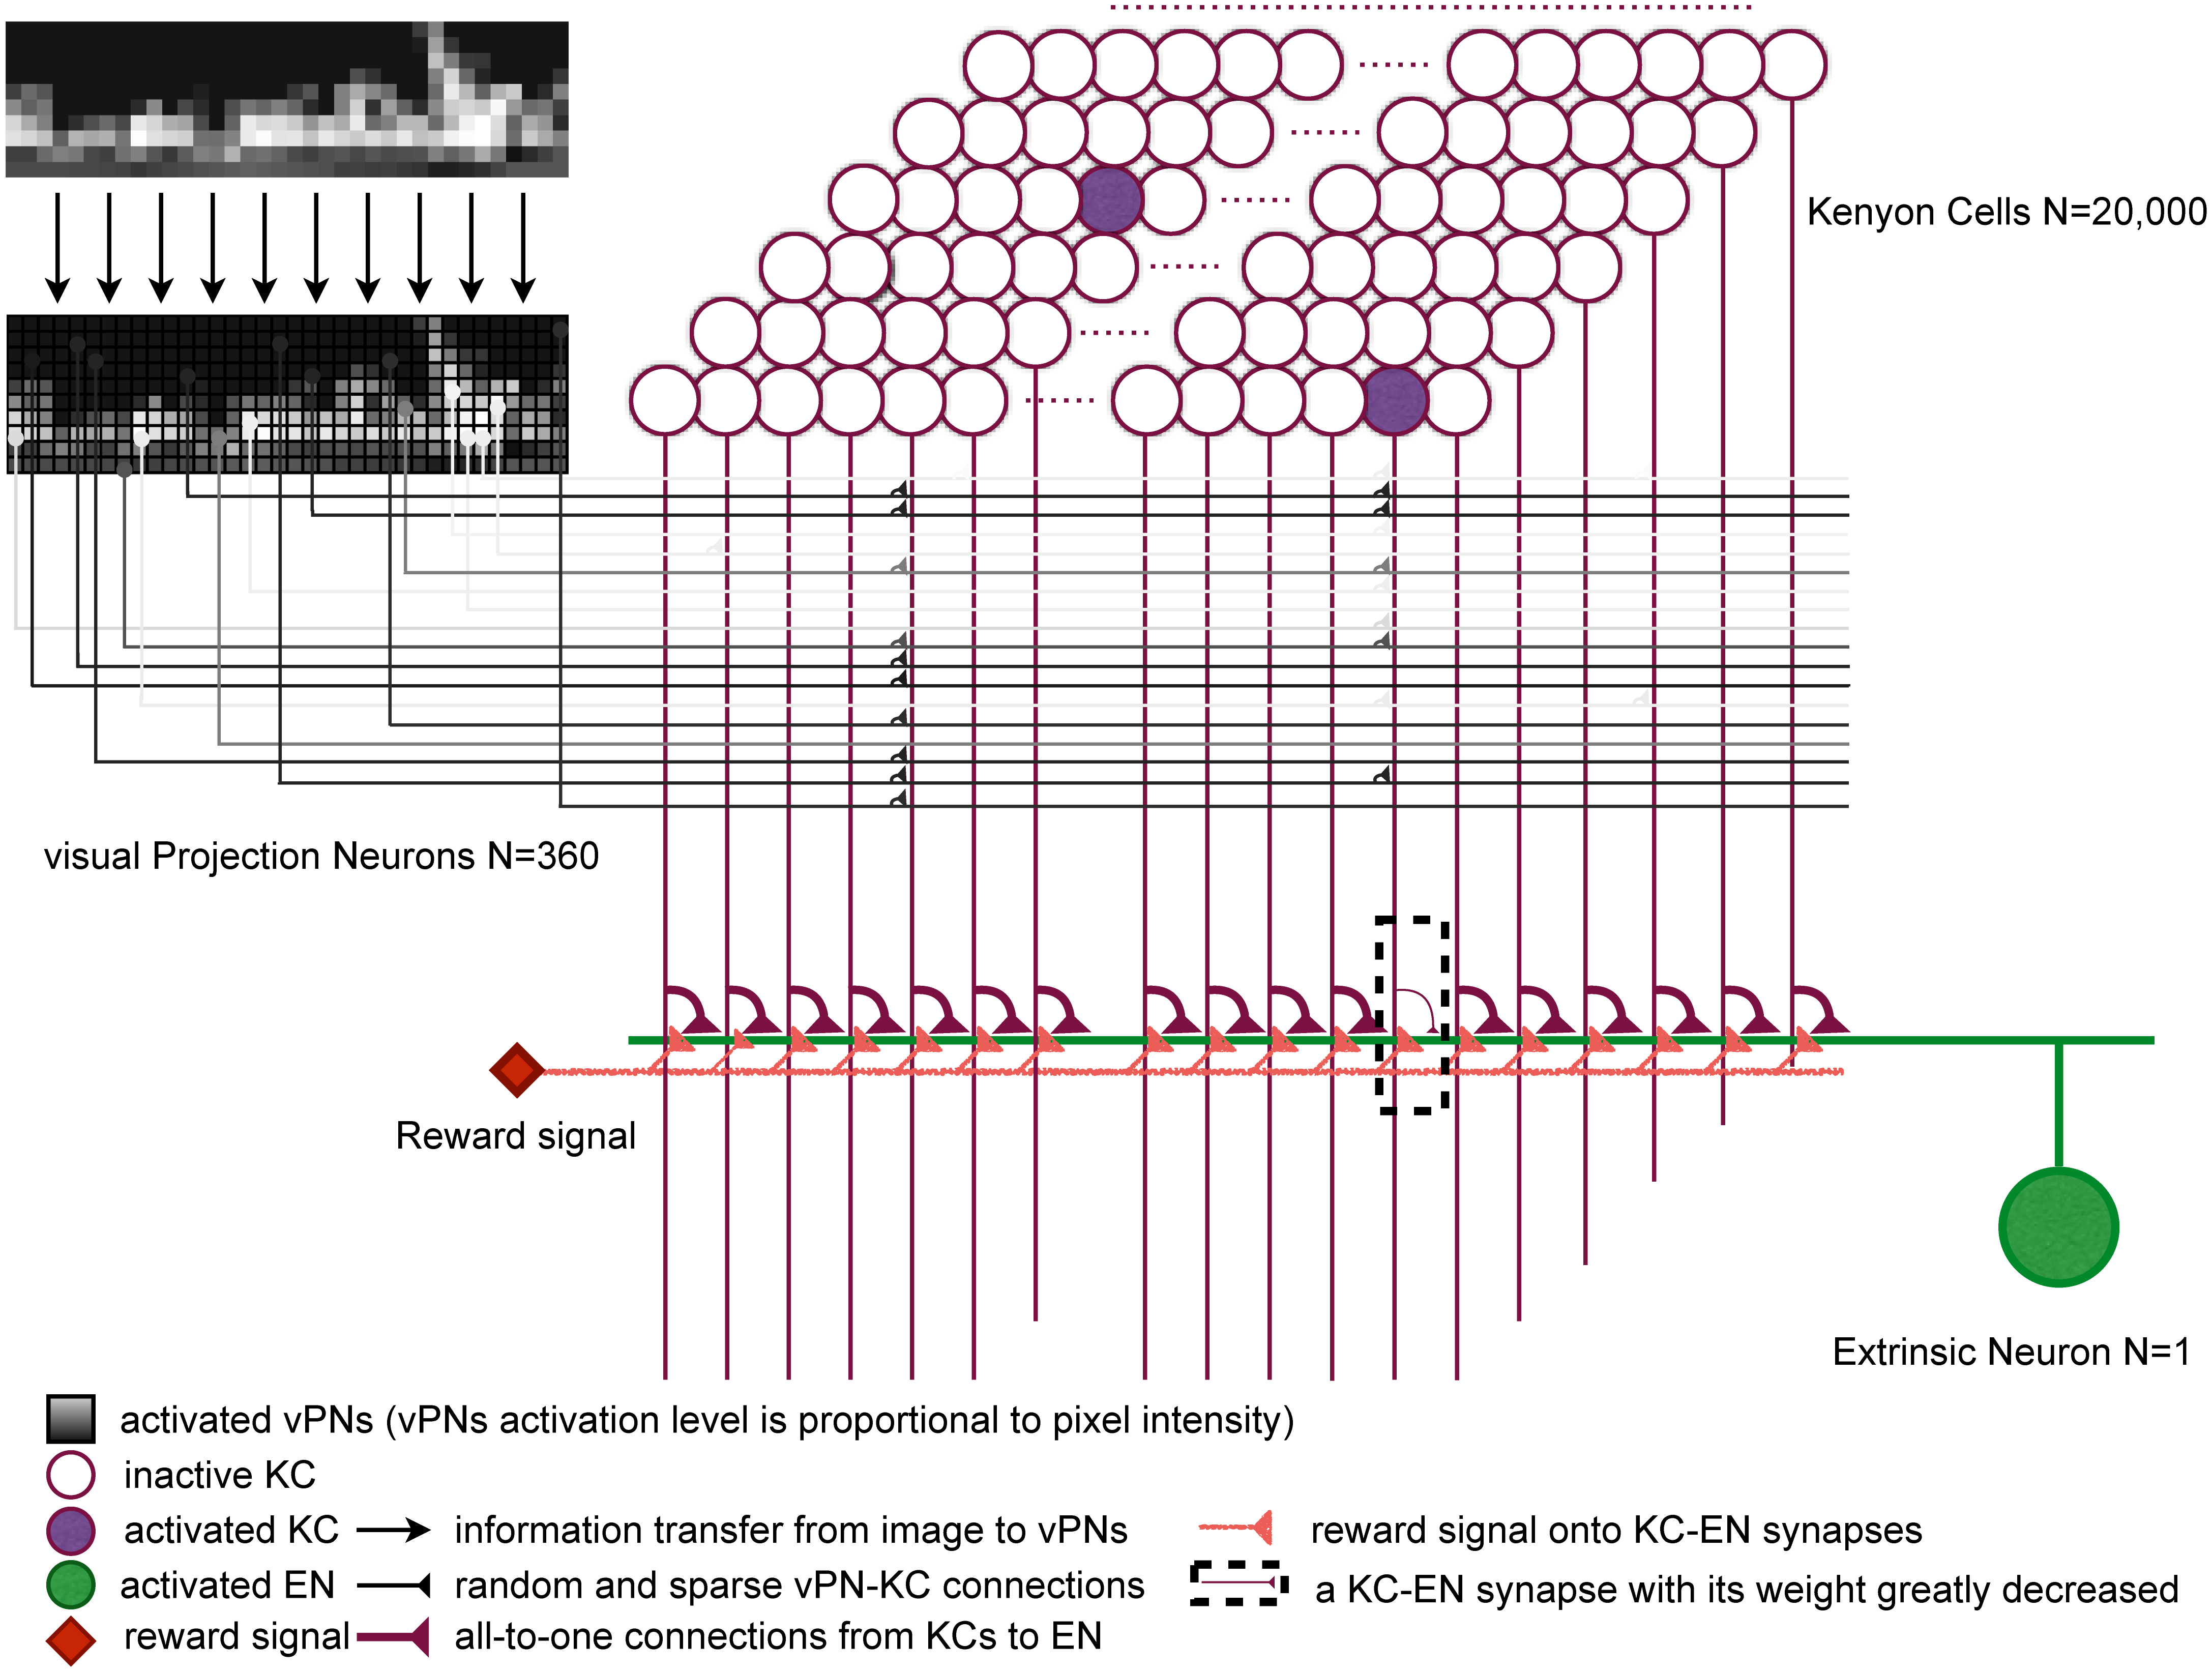
\includegraphics[width=0.9\textwidth]{Ardin2010MBModel}
  \caption{\label{fig:mb} The Mushroom Body circuit: (Caption from
    \textit{Ardin et al.}, Figure 2; note, their description and figure uses
    ``EN'' instead of ``MBON''): Images (see Fig 1) activate the visual
    projection neurons (vPNs). Each Kenyon cell (KC) receives input from 10
    (random) vPNs and exceeds firing threshold only for coincident activation
    from several vPNs, thus images are encoded as a sparse pattern of KC
    activation. All KCs converge on a single extrinsic neuron (EN) and if
    activation coincides with a reward signal, the connection strength is
    decreased. After training the EN output to previously rewarded (familiar)
    images is few or no spikes.}
\end{figure}

Learning occurs by showing patterns (images) to the vPNs. Each KC sums the
brightness of all connected vPNs and compares that sum to the activation
threshold. If the total brightness is greater than the threshold then the KC is
\textit{activated}. As the connections between the vPN and KC layers are random,
a given image will generate some sparse pattern of KC activation; to learn this
pattern, the weight of the KC-MBON connection is lowered from 1 to 0 for the
active KCs.
\newline
\par

To determine image familiarity during the recapitulation process, a pattern is
projected onto the vPNs (again giving a sparse pattern of KC activation).
The MBON then sums the synaptic (KC-MBON) weights of all active KCs to obtain a
\textit{familiarity} measure; recall, these weights are decayed as part of the
learning process; thus, the lower the MBON output, the more familiar the image
(and vice versa). Different route following strategies have been implemented:
scanning \cite{Ardin2016, Eberding2016, Zhang2017}, Klinokinesis
\cite{Zhang2017}, combination with the CX model \cite{Zhang2017}(see below), and
visual scanning \cite{Mitchell2018}). Most commonly, some form of scanning
is used whereby the agent scans an arc for the most familiar direction.
\newline
\par

This explanation has been a brief and is provided solely for context
as we do not work too closely with the MB though it is part of the
proposed model. Part 1 has more focus on visual navigation and gives
slightly deeper insight \cite{Mitchell2018} (particularly in relation
to AntBot projects), and of course the work of \textit{Ardin et al.}
can give the full details \cite{Ardin2016}.
\newline
\par

The MB model described above has been tested on the AntBot in three
different works (albeit using different methods and metrics); the
network as presented in \cite{Eberding2016, Zhang2017, Mitchell2018}
differs only in the number of PNs present (900 vPNs are used in all
three works, as opposed to the 360 present in \cite{Ardin2016}), and
the KC modelling (\textit{Ardin et al.} use a spiking
model\footnote{The AntBot projects do not explicitly model membrane
  potentials and realistic neural responses.  They use a simple
  abstraction for the sake of complexity. The network function is the
  same.} for the KCs \cite{Ardin2016}). More relevant to this work is
the modification given by \textit{Zhang}, whereby, 8 MBONs
are present as opposed to 1 (see Section \ref{CXMBBackground}).
\newline
\par

\subsection{ The Central Complex for Path Integration } \label{CXBackground}
The Central Complex (CX) is a highly conserved structure present in the insect
brain \cite{Pfeiffer2014, Stone2017}. Though the finer structural details and
component position may vary, the basic composition is more or less the same
across species \cite{Pfeiffer2014}. Organization and function of the
various parts of the CX are set out by \textit{Pfeiffer and Homberg} in
\cite{Pfeiffer2014}.
\newline
\par

We direct our attention to the CX model presented by \textit{Stone et
  al.}  which is the first neural model for path integration in the
insect brain with its structure drawn purely from insect
physiology. Interestingly, this model is a more advanced version of an
earlier model presented by \textit{Haferlach et al.}, which was
\textit{evolved} using a Genetic Algorithm \cite{Haferlach2007}. We
present this also, as it provides some historical context for the
development of a biologically plausible neural circuit for path
integration.

\subsubsection{The Evolved Model for Path Integration}
Prior to the CX model described below, there were several candidate
neural networks proposed for PI in ants
\cite{Haferlach2007}. \textit{Haferlach et al.}  report the two
best-known candidates being hand-designed, with more recent research
being directed towards an evolutionary approach to network design
\cite{Haferlach2007}. The approach presented in \cite{Haferlach2007}
follows this trend and employs a Genetic Algorithm (GA) (see Appendix
\ref{ap:ga} for a brief overview of GAs) to evolve a neural model
which is suitable for PI with biologically plausible inputs.
\newline
\par

\textit{Haferlach et al.} encode solutions as lists of integers. In these lists
there are \textit{start markers} and \textit{end markers} which delimit
the definitions of the actual neurons or sensors present in the model. The
complete model (topography, connection weights, sensors, and effectors) is
limited to a fixed-size encoding (genome limited to 500 parameters; ~$50$ neurons
maximum) \cite{Haferlach2007}. An example encoding from \cite{Haferlach2007} can
be seen in Figure \ref{fig:markerbasedencoding}.
\newline
\par


\begin{figure}[h!]
  \centering
  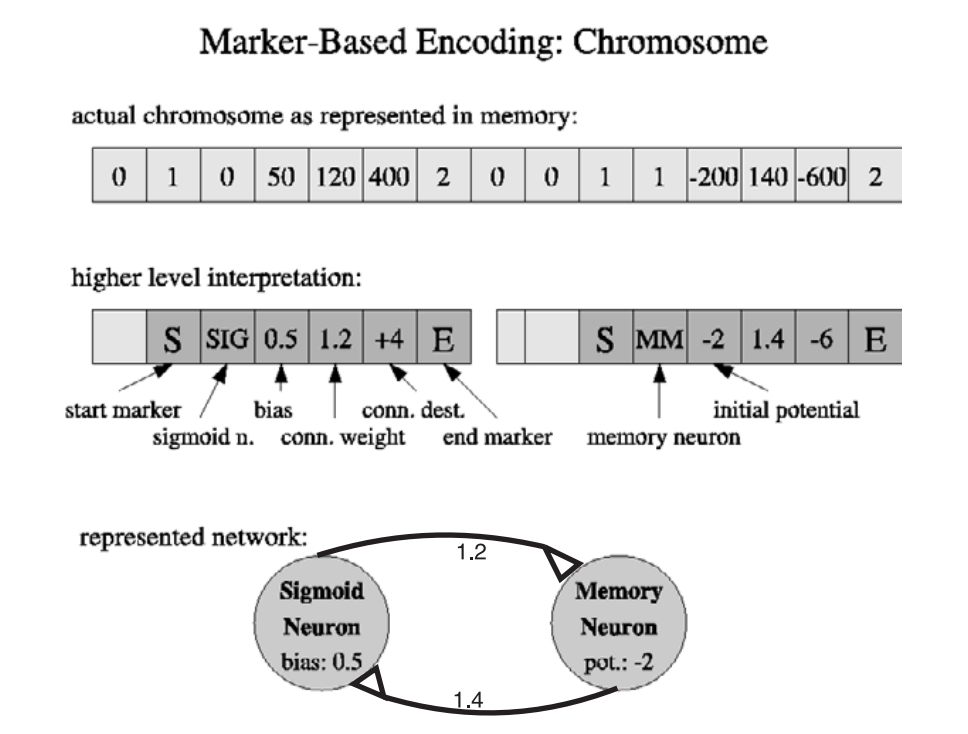
\includegraphics[width=0.9\textwidth]{MarkerBasedEncoding}
  \caption{\label{fig:markerbasedencoding} (Figure 2 from \cite{Haferlach2007})
    The Marker-Based encoding scheme used by \textit{Haferlach et al.},
    demonstrating how a simple neural model would be encoded as a sequence of
    integers.}
\end{figure}

Localised \textit{tournament selection} is used
to pick solutions for transition into the next generation. Each
solution is assigned a location in 1-dimensional space; a solution is
picked randomly, then another solution within distance $k$ of the
first is picked for the tournament ($k$ usually between 5 and 15)
\cite{Haferlach2007}. The solution with higher fitness wins the
tournament and progresses to mutation and
\textit{crossover}\footnote{Crossover - A particular method for
  breeding two solutions whereby their genomes are cut at a particular
  point and the ends swapped.}. This localised selection allows the
algorithm to find multiple \textit{good} solutions which need not
share the same genetic information.
\newline
\par

The fitness of each solution is evaluated by having the agent navigate
an outbound path through two randomly chosen points, then testing its
ability to navigate back to the start point. During the outbound
phase, information is input into the path integration network via the
sensors; the network output is ignored. During the inbound route, the
agent is steered by the network output.  An individual solution is
evaluated until some maximum time limit $m$ is reached, and the
distance to the start point $dist_t$ is computed at each time step. The
fitness is then the inverse sum of squared distances
\cite{Haferlach2007}:

\begin{equation}
 f = \frac{1}{\sqrt{\int_{0}^m dist_t^2 dt}}
\end{equation}

The fitness function is then augmented to penalise homeward routes which
spiral (circling the start point, getting closer with each pass), and
to reward networks which are simple in structure; shown in
Equations \ref{eq:fithead} and \ref{eq:fitsimple} respectively.

\begin{equation}
  \label{eq:fithead}
  f = \frac{1}{\sqrt{\int_{0}^m dist_t^2 |\theta - \omega | dt}}
\end{equation}
\begin{equation}
  \label{eq:fitsimple}
  f = \frac{1}{(1 + k_n)^{c_n}(1 + k_c)^{c_c}
    \sqrt{\int_{0}^m dist_t^2 |\theta - \omega | dt}}
\end{equation}

where $\omega$ is the nest heading, $\theta$ is the agent's heading,
$k_n$ is a neuron penalty constant, $k_c$ is a connection penalty
constant, $c_n$ is the number of neurons, and $c_c$ is the number of
connections (i.e.  the network is heavily penalised for the number of
connections and neurons it has, forcing simpler networks)
\cite{Haferlach2007}. These are applied as a two-stage evolutionary
process; evolve a solution first using Equation \ref{eq:fithead} to
compute the fitness, then use an optimum solution from the previous
stage to seed a new population and evolve a solution from here using
Equation \ref{eq:fitsimple}. The two-stage evolutionary process alone
did not find acceptable solutions. The search space was constrained by
providing the following four constraints on network topology:

\begin{itemize}
\item{each direction cell had to be connected to at least one memory neuron;}
\item{each direction cell had to be connected to at least one sigmoid neuron;}
\item{sigmoid neurons had to be connected to turn effectors;}
\item{a maximum of two turn effectors (left and right) were allowed
  \cite{Haferlach2007}.}
\end{itemize}


\textit{Haferlach et al.} present the model shown in Figure
\ref{fig:evolvednetwork}; notice the evolved structure bears a striking
resemblance to the CX model presented by \textit{Stone et al.} (Figure
\ref{fig:cx}). Indeed, this network operates on the same principle; encoding
a heading vector across multiple neurons with directional preferences. This
network provides a compact, elegant, robust model capable of performing
path integration with reasonable errors. The network also demonstrated
some capability for PI with obstacles present (though errors were generally much
greater) \cite{Haferlach2007}.

\begin{figure}[h!]
  \centering
  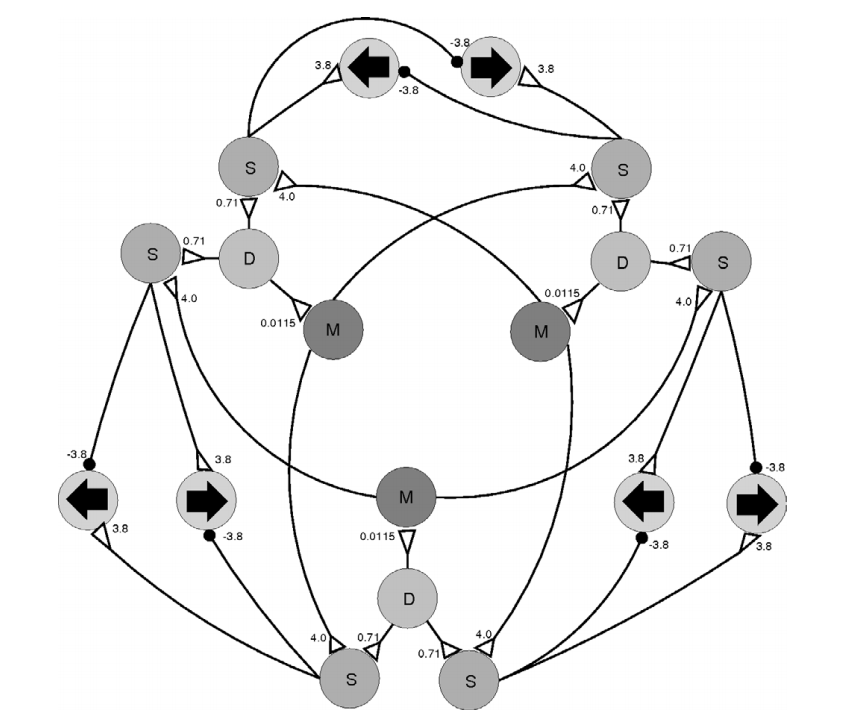
\includegraphics[width=0.7\textwidth]{EvolvedNetwork}
  \caption{\label{fig:evolvednetwork} (Figure 3 from \cite{Haferlach2007})
    The high-fitness network, consistently evolved using the constrained
    two-stage evolution process illustrated by \textit{Haferlach et al.}
  }
\end{figure}

\subsubsection{The Central Complex Model}
The Central Complex model is a six layer artificial neural network
presented by \textit{Stone et al.} which has been shown to provide a
plausible neural substrate for Path Integration (PI) both in
simulation and on the AntBot platform \cite{Scimeca2017,
  Stone2017}. The model presented is shown in Figure
\ref{fig:cx}. Splitting the model into its six layers, we can observe
a breakdown of functionality:
\newline
\par

\begin{itemize}
\item{Layer 1: Heading preprocessing (TL), Speed (TN)}
\item{Layer 2: Heading preprocessing (CL1)}
\item{Layer 3: Heading (TB1)}
\item{Layer 4: Memory (CPU4)}
\item{Layer 5: Normalisation and Inhibition (Pontine Neurons)}
\item{Layer 6: Steering/output (CPU1)}
\end{itemize}

\begin{figure}[h!]
  \centering
  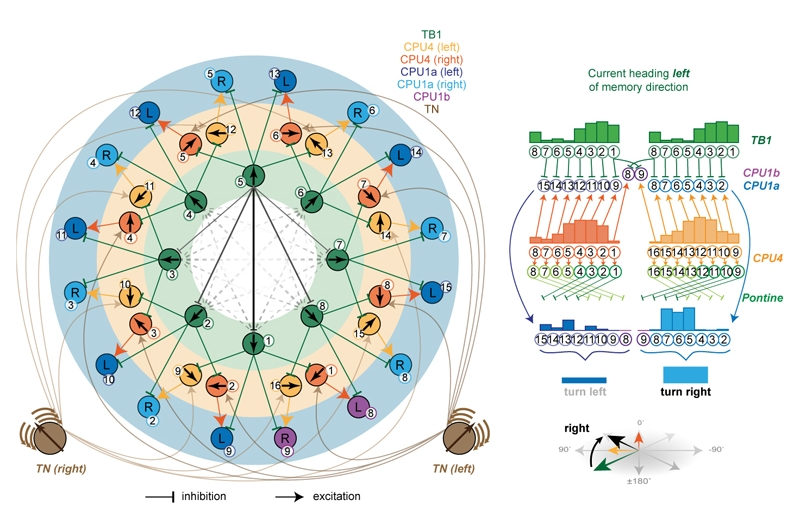
\includegraphics[width=\textwidth]{StoneCXModel}
  \caption{\label{fig:cx} The Central Complex model presented by
    \textit{Stone et al.}. (Left) This graph demonstrates the basic structure of
    the CX model (Figure 5G from \cite{Stone2017}). Pontine neurons have been
    excluded for clarity.
    (Right) This graph shows how signals propogate through the network where the
    current heading lies to the left of the desired heading, i.e. a right turn
    should be generated (Figure 5I from \cite{Stone2017}). The numbers given at
    each layer on the right correspond to the numbers given for each neuron
    in the graph on the left.
  }
\end{figure}

Figure \ref{fig:cx} shows four types of neuron: TN (Tangential Neuron,
brown), TB1 (green), CPU4 (yellow and orange), and CPU1 (dark blue,
light blue, and purple).
\newline
\par

While Figure \ref{fig:cx} (Left) distinguishes between CPU1a (blue) and
CPU1b (purple) neurons, we will ignore this distinction; for clarity, the
physiological mapping between these CPU1 subtypes in the Upper Central Body (CBU)
and the Protocerebral Bridge (PB) is different, but the function they serve in
the Central Complex is the same \cite{Stone2017}; thus, the distinction makes
no difference in the model. Similarly the normalisation and inhibition functions
of the Pontine Neurons only has an effect when the agent experiences holonomic
motion (motion where the view direction does not match the direction of travel);
as AntBot is incapable of such motion, we can safely ignore the function of
the Pontine Neurons; in our case, the Pontine Neurons would have the
same activity patterns as the CPU4 neurons \cite{Stone2017}. Figure \ref{fig:cx}
(Right) shows how the Pontine inhibition is structured.
\newline
\par

\begin{figure}[h!]
  \centering
  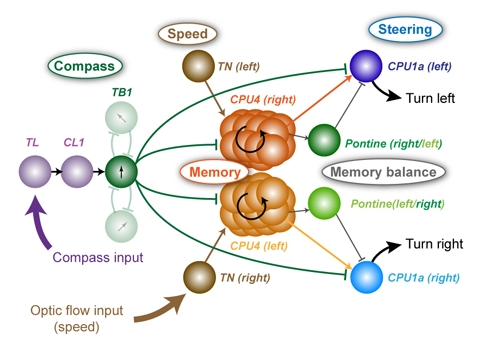
\includegraphics[width=0.7\textwidth]{Figure5F}
  \caption{
    \label{fig:cxlayer} Here we can see the layers of the CX model and
    how they fit together. A heading signal is input to the TL neurons,
    propogating through the CL layer to TB1 (heading ring-attractor) and
    CPU4 (memory). TN neurons (speed sensitivity) input directly to CPU4.
    So, the combination of heading and speed inputs to CPU4 gives a measure
    of distance travelled in a particular direction; this facilitates generation
    of a steering command in CPU1 providing a mechanism for path integration.
  }
\end{figure}

We now break down the different neuronal types and their proposed functions.
Citation is given, but for the avoidance of any doubt, the following descriptions
are adapted from \textit{Stone et al.} (see STAR Methods) \cite{Stone2017}.
We also add implementation information for the AntBot where appropriate;
occassionally the AntBot implementations are slightly different.
\newline
\par

\textbf{Simulated Neurons:}
Each neuron is described by its firing rate, where the firing rate $r$ is
a sigmoid function of the input $I$:

\begin{equation}\label{eq:sig}
r = \frac{1}{1 + e^{-(aI - b)}}
\end{equation}

where $a$ and $b$ are parameters which control the slope and offset of
the sigmoid function \cite{Stone2017}. Optionally, Gaussian noise may
be added to the output (no noise is applied in AntBot
implementations). The input to each neuron is the weighted sum of the
activity of each neuron that synapses onto it; say neuron $j$, the
input is:

\begin{equation}
  I_j = \sum_{i} w_{ij} \cdot r_i
\end{equation}

The weights used by \textit{Stone et al.} can only be 0, 1, or -1 for
no-connection, excitatory, or inhibitory respectively \cite{Stone2017}.
\newline
\par

% Function of CL & TL
\textbf{TL \& CL1:}
The TL neurons are the input point for heading information. In the ant brain
this heading information comes from a \textit{sky-compass}; the ant eye contains
cells sensitive to polarized light which allows the ant to infer an accurate
allothetic heading from vision alone. Interestingly, there is also evidence that ants
have the capability to infer a direction without a view of celestial cues,
suggesting they may have access to some other signal, the candidate signal being
the geomagnetic field \cite{Fleischmann2018, Grob2017}. The TL neurons have been
shown to be polarisation sensitive across multiple insect species \cite{Stone2017}
(see STAR Methods). Each TL neuron has a preferred direction (i.e. a specific
direction of poliarisation sensitivity) $\theta_{TL} $, and there are 16 such
neurons representing the 8 directions around the agent (i.e.
$\theta_{TL} \in \{ 0^{\circ}, 45^{\circ}, 90^{\circ}, 135^{\circ}, 180^{\circ},
225^{\circ}, 270^{\circ}, 315^{\circ}\} $) \cite{Stone2017}. Together, the 16
TL neurons encode the heading of the agent in a single timestep; each neuron
receives input activation as:

\begin{equation}
  I_{TL} = \cos ( \theta_{TL} - \theta_{h} )
\end{equation}

where $\theta_{TL} $ is the preferred heading of the neuron as above, and
$\theta_{h} $ is the current heading of the agent. In the next heading layer,
there are 16 CL1 neurons which use inhibition to invert the polarisation
response \cite{Stone2017}. \textit{Stone et al.} comment that these neurons
effectively make no difference to the model and are included for completeness.
They are also included in previous AntBot projects which make use of the CX model
\cite{Zhang2017, Scimeca2017}. On AntBot, the heading is derived from the onboard
compass on the mobile phone (see Section \ref{sec:platform}).
\newline
\par

% Function of TN
\textbf{TN:}
There are 4 TN neurons which act as an input for speed information. The TN
neurons are sensitive to optical flow and can be split into two subtypes:
TN1, and TN2. \textit{Stone et al.} showed that TN1 neurons are inhibited by
simulated forward flight and excited by simulated backward flight, while TN2
neurons are inhibited by simulated backward flight and excited by simulated
forward flight \cite{Stone2017}. Each of the four TN neurons has a tuning
preference; these tuning preferences were measured in bees as approximately
$+45^{\circ}$/$-45^{\circ}$ for TN2, and $+135^{\circ}$/$-135^{\circ}$ for TN1
(where $0^{\circ}$ is straight ahead). In summary, we have TN$1_{left}$,
TN1$_{right}$, TN$2_{left}$, and TN$2_{right}$. It is thought that these neurons
provide a (or part of a) mechanism for odometry by allowing the model to
integrate speed with respect to time giving a distance measure \cite{Stone2017}.
\textit{Stone et al.} give the speed calculation from the TN neurons
as:

\begin{equation}
  I_{TN_{L}} =
  [ \sin (\theta_{h} + \phi_{TN}) \quad \cos (\theta_{h} + \phi_{TN}) ]\mathbf{v}
\end{equation}

\begin{equation}
  I_{TN_{R}} =
  [ \sin (\theta_{h} - \phi_{TN}) \quad \cos (\theta_{h} - \phi_{TN}) ]\mathbf{v}
\end{equation}

where $\mathbf{v}$ is the velocity of the agent in Cartesian coordinates,
$\theta_h \in [0^{\circ}, 360^{\circ})$ is the current heading of the agent, and
$\phi_{TN}$ is the preferred angle of that TN neuron \cite{Stone2017}.
\newline
\par

The TN neurons are not modelled in the \textit{basic} CX model on AntBot. There
is, however, a \textit{holonomic} implementation which models both the TN1 and
TN2 neurons present on the robot. The formulae above are implemented on the
robot but they are never used. Instead, the raw left and right speeds computed
from the optical flow are passed in (see \textit{Scimeca} \cite{Scimeca2017} for
the details of speed computation from optic flow). The TN2 neurons will simply
clip these speeds to make sure they lie in $[0,1]$; the TN1 neurons will perform
$(1 - s) / 2$ for both the left and right speeds $s$, then clip the output to lie
in $[0,1]$. The output is returned directly, rather than being returned as a
sigmoid (as for all other neuron types).
\newline
\par

% Function of TB1
\textbf{TB1:}
There are eight TB1 neurons, each with a directional preference $\theta_{TB1}$,
which correspond to the eight cardinal directions in the model. Each TB1 neuron
receives excitatory input from the pair of CL1 neurons that have the same
directional preference. The TB1 layer contains inhibitory connections between
peer neurons where each TB1 neuron strongly inhibits other TB1 neurons with
opposite directional preferences (see Figure \ref{fig:cx}) forming a
\textit{ring attractor}\cite{Stone2017}. The weighting for an arbitrary
inhibitory connection from neuron $i$ to neuron $j$ is given by:

\begin{equation}
  w_{ij} =
  \frac{\cos (\theta_{TB1,i} - \theta_{TB1,j}) - 1}{2}
\end{equation}

where $\theta_{TB1,i}$ is the direction preference of TB1 neuron $i$ (similarly
for $\theta_{TB1,j}$). The total input for each TB1 neuron from the CL1 layer
at timestep $t$ is:

\begin{equation}
  I_{TB1_{j}^{(t)}} =
  (1 - c) \cdot r_{CL1_j}^{(t)} + c \cdot \sum_{i = 1}^{8} w_{ij}
  \cdot r_{CL1_j}^{(t - 1)}
\end{equation}

where $c = 0.33$ is a scaling factor which determines the relative strength
of excitation from the CL1 layer and inhibition from other TB1 neurons;
the AntBot implementation of the TB1 neurons is the same. This
network layer produces a stable heading encoding which provides accurate
input for the CPU4 layer, underpinning accurate path integration.
\newline
\par

% Function of CPU4
\textbf{CPU4:}
The 16 CPU4 neurons receive input in the form of an accumulation of
heading $\theta_h^{(t)}$ of the agent, along with a modulated speed response
from the TN2 neurons \cite{Stone2017}. The CPU4 neurons accumulate distance with
direction. The input the CPU4 neurons is given by:

\begin{equation}
  \label{eq:cpu4update}
I_{CPU4}^{(t)} = I_{CPU4}^{(t - 1)} + h \cdot (r_{TN2}^{(t)} - r_{TB1}^{(t)} - k)
\end{equation}

where $h = 0.0025$ determines the rate of memory accumulation, and $k = 0.1$ is
a uniform rate of memory decay \cite{Stone2017}. All memory cells are initialised
to $I_{CPU4}^{(0)} = 0.5$ and are clipped at each timestep to fall between 0 and
1 \cite{Stone2017}. As shown in Figure \ref{fig:cx}, each TB1 provides input to
two CPU4 neurons, each of which receives input from the TN2 cell in the opposite
hemisphere. As these neurons accumulate distance with respect to a direction,
they provide a population encoding of the \textit{home vector} (the integrated
path back to the nest) \cite{Stone2017}. Interestingly, \textit{Zhang} showed
that the network can be initialised to an arbitrary state, allowing the agent
to navigate along arbitrary vectors \cite{Zhang2017}. While this seems intuitive,
the experimental evidence is valuable and demonstrates that the CPU4 layer could
form a basis for the \textit{vector memory} discussed by \textit{Webb} in
\cite{Webb2019} (see Section \ref{CXMBBackground}).
\newline
\par

The basic CX model on the AntBot does not model TN neurons, so the input is
computed differently; furthermore, the gain and loss factors are different.
The input can be expressed as:

\begin{align}
  I_{CPU4}^{(t)} =
  I_{CPU4}^{(t - 1)} + s \cdot ((1 - r_{TB1}^{(t)}) \cdot g - l)
\end{align}

where $l = 0.0026$ is the uniform rate of memory loss, $g = 0.005$ is the
uniform rate of memory gain, and $s$ is the current speed. This value is
then clipped to lie in $[0,1]$. As an aside, in the holonomic model
mentioned previously, the input is computed as in Equation \ref{eq:cpu4update}
as the TN neurons are present in the model.
\newline\par

\textbf{Pontine:}
The pontine neurons project contralaterally connecting opposite CBU columns
(shown in Figure \ref{fig:cx} (Right)). The 16 pontine neurons each receive input
from one CPU4 column \cite{Stone2017}; pontine input can be given simply as:
\newline
\par

\begin{equation}
  I_{Pontine}^{(t)} = r_{CPU4}^{(t)}
\end{equation}

The pontine neurons are not implemented on AntBot for simplicity. AntBot is
incapable of holonomic motion, so they would have no functional effect.
\newline
\par

% Function of CPU1
\textbf{CPU1:}
There are 16 CPU1 neurons present in the model. Each of which
receives inhibitory input (weight $= -1$) from a TB1 neuron; where, each
TB1 neuron provides inhibitory input to two CPU1 neurons (in the same pattern
as the TB1-CPU4 connections - see Figure \ref{fig:cx}). Each CPU4 neuron also
provides input to a CPU1 neuron (so we get input from vector memory and current
heading). The CPU1 input can be expressed as:

\begin{equation}
  I_{CPU1}^{(t)} = r_{CPU4}^{(t)} - r_{Pontine}^{(t)} - r_{TB1}^{(t)}
\end{equation}

As can be seen the CPU1 neurons also receive input from the pontine neurons.
The CPU1 neurons form two sets, those connecting to left motor units and those
connecting to the right. On AntBot the pontine term is omitted
(i.e. the input becomes
$I_{CPU1}^{(t)} = r_{CPU4}^{(t)} - r_{TB1}^{(t)}$).
\newline
\par

We choose a direction simply by summing the CPU1 outputs on both sides
and the difference indicates the direction and strength of the
required heading correction:

\begin{equation}
  \theta_h^{(t)} = \theta_h^{(t - 1)} +
  m \cdot (\sum_{i = 1}^{8} r_{CPU1R_{i}} - \sum_{i = 1}^{8} r_{CPU1L_{i}})
\end{equation}

where $m = 0.5$ is a constant \cite{Stone2017}. The angle computation is the
same on the AntBot.
\newline
\par

There are some details which have been omitted for clarity. The stack
presented here should effectively describe how the network generates a
turning signal from its current state and inputs to perform effective,
accurate path integration. For further details, please consult
\cite{Stone2017} (the STAR Methods section contains the full technical
details of the model).

\subsection{ The Eight MBON Model (CXMB) } \label{CXMBBackground}
In \cite{Zhang2017}, the MB network is modified by adding 7 MBONs. Each MBON has
its own KC-MBON connection array, each with their own unique weights. Each
connection array corresponds to one of the eight cardinal directions represented
by the TB1 layer of the CX model (namely, $0^{\circ}$, $45^{\circ}$,
$90^{\circ}$, $135^{\circ}$, $180^{\circ}$ ,$225^{\circ}$, $270^{\circ}$,
$315^{\circ}$) (see Section \ref{CXBackground}).
\newline
\par

The additional MBONs give image memory an associated direction, so
training is performed with respect to orientation. For example, if the
agent has a heading of $45^{\circ}$ when a image is stored, then only
the corresponding connection array has its weights updated during
learning. Practically, this is done by querying the TB1 layer of the
CX model to find the current direction according to the model (rather
than directly querying the robot's onboard compass directly). This
process is visualised in Figure \ref{fig:eightmbon}.
\newline
\par

\begin{figure}[h!]
  \centering
  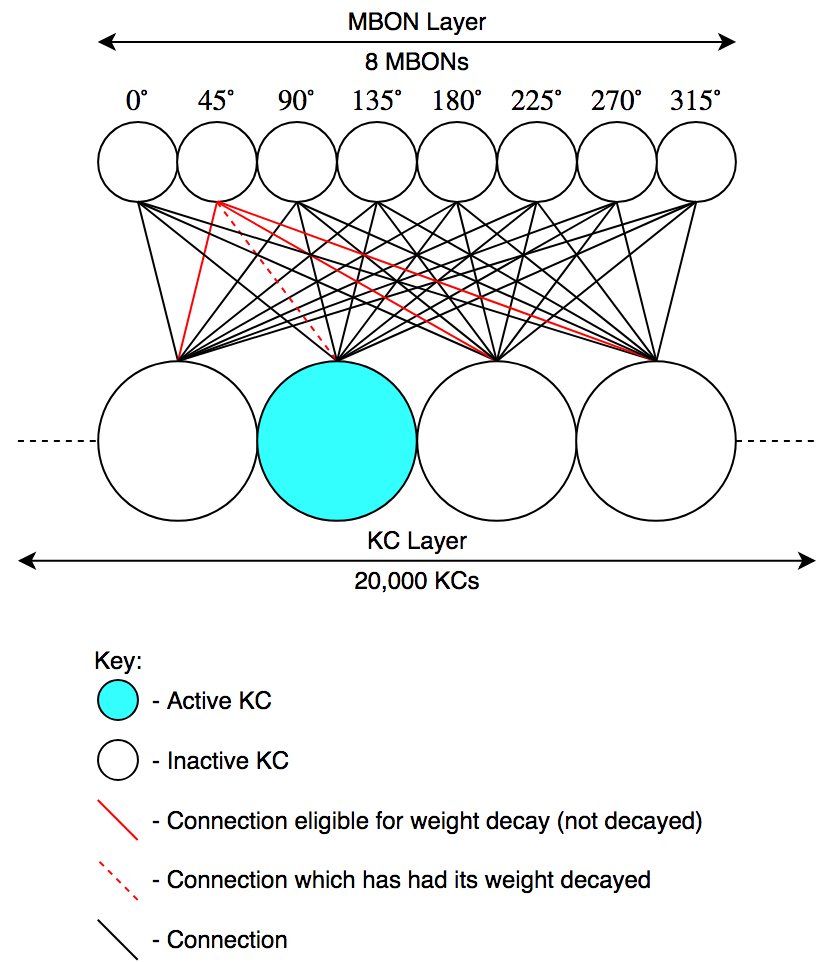
\includegraphics[width=0.9\textwidth]{EightENModel}
  \caption{\label{fig:eightmbon} Our interpretation of the eight MBON model
    proposed by \textit{Zhang}. Every KC connects to every MBON. All connection
    weights start out at $w=1$. Following the example presented in the text,
    if an image being learned corresponds to facing a direction of $45^{\circ}$,
    then only the conncetions to that MBON (highlighted in red) are eligible to
    have their weights modified. Recall, however, that these weights will only
    be modified if the KC was activated (not shown in the figure).
    }
\end{figure}

While, in theory, this eight MBON model could function independently,
\textit{Zhang} uses it to (rather neatly) augment the CX model
(creating the combined CXMB model); this allows navigation to be
performed using a combination of visual memory and path integration
information. The navigation process can be described by a sequence of
equations. We modify the notation slightly for clarity, but the
equations are the same as presented in \cite{Zhang2017}.
\newline
\par

During recall, the MB circuit is shown an image in the usual way (see
Section \ref{MBBackground}); however, we now get eight responses,
giving us a response distribution. This distribution can be
interpreted as giving us the most likely direction of travel, when the
image presented was first observed. This distribution requires some
modification to integrate it into the CX response. Let $M_i$ be the
familiarity response of the $i$th MBON; the responses are normalised
as:

\begin{equation}
  \bar{M}_i = \frac{M_i}{\Sigma^{8}_{k = 0} M_k}
\end{equation}

which gives us the normalised response $\bar{M}_i$ between 0 and 1. $\bar{M}_i$
must be inverted so that the most likely direction has the greatest response
(in the MB model, the most familiar direction would give the lowest response):

\begin{equation}
  \bar{M}^{-1}_i = 1 - \bar{M}_i
\end{equation}

This visual response is then combined with the memory response from the CPU4
layer of the CX model to give output at the CPU1 layer:

\begin{equation}
  CPU1_{output} = k \cdot W_{CPU4} \cdot CPU4 + (1 - k) \cdot W_{MBON} \cdot
  \bar{M}^{-1}
\end{equation}

where $k$ is a weighting factor that determines the relative stregths of the CX
response and the MB response in the output ($k = 0.8$ in \cite{Zhang2017}),
$\bar{M}^{-1}$ is the collection of all inverse normalised MBON responses,
$W_{CPU4}$ is a custom matrix\footnote{This is the term used by \textit{Zhang} to
  describe   the $W_{CPU4}$ matrix. More specifically, this matrix describes the
  connections between the CPU4 and CPU1 layers of the CX model.}, $W_{MBON}$ is
an identity matrix that will expand the MBON response array from 8x1 to 16x1
\cite{Zhang2017}.
\newline
\par

In order to test the CXMB model, \textit{Zhang} first demonstrated the
functionality of a \textit{copied memory model}. The test of the
copied memory model aimed to prove that the CPU4 state of the agent
could be copied and stored, the CPU4 state modified, and then restored
from the copy to allow the agent to navigate home. The copied memory
model was tested by sending the agent on a pre-determined oubound
route to a feeder (chosen at random, but consistent between trials),
copying the CPU4 state, and allowing the robot to navigate home using
the CX model; the CPU4 state will be modified by this homeward
navigation.  The agent is then replaced at the feeder, its CPU4 state
restored from the copy, and tasked with navigating home a second
time. The copied memory model was tested as a pre-requisite for
testing the CXMB model, however, it demonstrates an important
capability of the CX model; namely, the capability to directly load a
state into its memory in order to navigate; a concept referred to as
\textit{vector memory} in \cite{Webb2019}. Indeed, this concept of
vector memory is shown to be quite a useful tool in insect navigation
\cite{Webb2019}. At time of writing, the precise biological mechanism
employed by insects to perform this task is unknown.
\newline
\par

The CXMB model is then tested in the same way. The agent follows its oubound
route to the feeder, navigates back once using the CX model (the MB model is
trained on this first inbound trip), is replaced at the
feeder, and finally, tasked with navigating back again, this time using the CXMB
model. To be clear, the CPU4 state of the CX model is stored after the outbound
route, and loaded back into the network before the second inbound trip.
\textit{Zhang} reports that the second inbound trip (using both CXMB) showed
more heading adjustments during its traversal and, on average, performed
slightly better than a pure CX implementation\cite{Zhang2017}. It should also
be noted that the average performance of both models in \textit{Zhang's} work
was good \cite{Zhang2017}.
\newline
\par

We note two methodological problems with \textit{Zhang's} work: The outbound
route, while randomly chosen, was the same across all trials, and, for the
copied memory and CXMB experiments, the agent was placed facing the nest for
the test run (second inbound). To add to the first problem, the outbound route
ended such that the robot was facing back towards the nest. Both of these flaws
could lead to apparent path integration behaviour where, in fact, the agent
could have made it sufficiently close to the nest by simply following a straight
line. While the agent was certainly employing the CX to perform path integration,
we do not feel that the tests chosen provide strong evidence of functionality.

\subsection{ Review of Part 1 }
The work in \cite{Mitchell2018} specifically covers the Mushroom Body
and Optical Flow Collision Avoidance. The Mushroom Body model used in
\cite{Mitchell2018} is the same as that used by \textit{Ardin et al.} in
\cite{Ardin2016}, except for the small differences noted in Section
\ref{MBBackground}. The model tested in \cite{Mitchell2018} used a single MBON
with a scan-based route following strategy. The scanning differed from previous
works as it was implemented as an image manipulation algorithm (termed
\textit{visual scanning}) instead of a physical turn performed by the AntBot.
\newline
\par

Multiple OFCA systems were tested, however in final experiments an
optical flow filtering system is used (see Section
\ref{sec:offbg}). This strategy proved simple, but effective. While we
initially move away from it for this project, it was used for
initial tests of the CX model, as it provided a simple out-of-the-box
method to generate a non-deterministic path for the model to
integrate.
\newline
\par

Both systems functioned well and provided a solid baseline from which we will
work in this project. The MB model proved very capable at following routes
learned in a non-deterministic fashion through a cluttered environment.
\newpage

%%%%%%%%%%%%%%%%%%%%%%%%%%%%%%%%%%%%%%%%%%%%%%%%%%%%%%%%%%%%%%%%%%%%%%%%%%%%%%%
% PLATFORM                                                                    %
%%%%%%%%%%%%%%%%%%%%%%%%%%%%%%%%%%%%%%%%%%%%%%%%%%%%%%%%%%%%%%%%%%%%%%%%%%%%%%%
% High level description of the platform. This section can be short. Refer back
% to Part 1 for detail.
\section{ Platform } \label{sec:platform}
The AntBot is an autonomous robot built to allow easy testing of the
various navigational algorithms in the \textit{Ant Navigational Toolkit}
on a physical agent. AntBot is assembled using off-the-shelf parts with an
Android phone at its heart. We give a high level description here; additional
detail can be found in \cite{Mitchell2018}.

\subsection{ Hardware }
The robot is composed of three main parts: a Dangu Rover 5 chassis, an
Arduino microcontroller, and a Google Nexus 5 Android smartphone. The
smartphone provides a (theoretically) solid base for an autonomous
agent, with sufficient processing power and memory to run the models,
a convenient touchscreen interface to display information and an
adaptable control interface, a built-in camera, and extensive software
libraries. As such, the smartphone works as the computational centre,
performing all higher sensory processing and acting on this analysis.
Once the algorithm running on the phone has decided on a course of
action, it sends a command via a serial connection to the Arduino
board; the board, then parses the command and translates it into a
sequence of motor commands which are sent to the built-in motor board
in the chassis.\newline\par
\begin{figure}[h!]
  \centering
  \includegraphics[width=0.7\textwidth]{AntBotCharging}
  \caption{
    \label{fig:antbotcomp} The AntBot, connected to the charging station.
    This figure also shows the position of the mobile phone, camera attachment,
    and retroflective motion capture markers on the top of the robot.
    }
\end{figure}

Additionally, the robot possesses a $360^{\circ}$ camera attachment, giving the
robot a panoramic view to match that of the desert ant\footnote{In reality,
  the desert ant has a visual field of only ~$280^{\circ}$\cite{Ardin2016},
  however an approxmiation of $360^{\circ}$ was considered appropriate when
  the robot was built.}. The robot was also modified as part of
\cite{Mitchell2018} to allow it to be charged with an external charger without
dismantling it.

\begin{figure}[t!]
  \centering
  \begin{minipage}[t!]{0.45\textwidth}
    \centering
    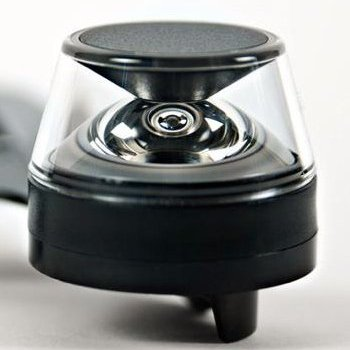
\includegraphics[width=0.9\textwidth]{KogetoDot}
    \caption{The Kogeto Dot 360$^\circ$ panoramic lens attachment.}
  \end{minipage}
  \hfill
  \begin{minipage}[t!]{0.45\textwidth}
    \centering
    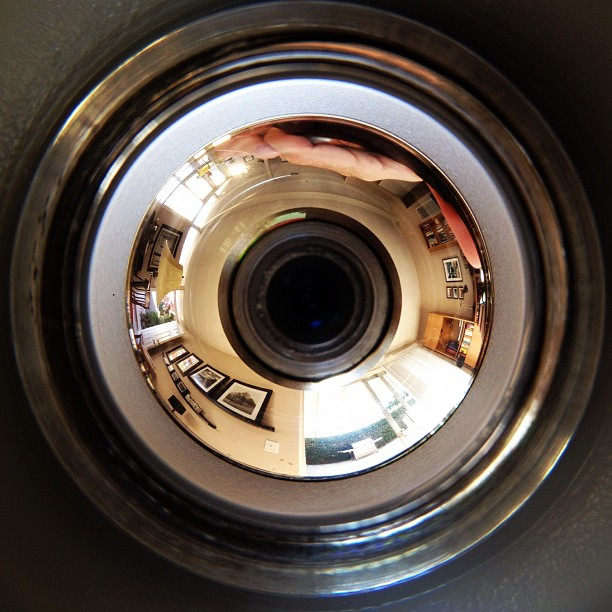
\includegraphics[width=0.9\textwidth]{PanoramicView}
    \caption{A sample view of the lens from the front facing camera, before any
      processing.}
  \end{minipage}

\end{figure}

\subsection{ Software }
The robot requires two levels of software; higher level Java (Android) code to
perform the high level functions and lower level code written in C/C++
(Arduino dialect). The Arduino code can be thought of as the firmware.

\subsubsection{ Android } \label{subsubsec:droid}
Android provides a reasonable conceptual basis for working on robotics
projects. The Operating System permits multiple applications to run
asynchronously and pass information between them; for example, the
user could develop an application to perform all visual processing
then broadcast a processed image for other applications which require
it. The original AntBot software was split into separate five
applications: Ant Eye, Visual Navigation, Path Integration, Combiner,
and Serial Communications, neatly compartmentalising each task.
In recent years, this structure appears to have been abandoned and
almost all code is contained within the \textit{AntEye}
application. Only the Serial Communications application remains
true-to-design.
\newline
\par

Typical flow within AntEye will see an image captured from the front camera,
processed such that we get a downsampled 90x10 image which represents the
$360^{\circ}$ view around the robot. This image is then used for optical
flow analysis. The image and flow analysis are then made available to any thread
which requires it. A thread will then use this data to run an experiment.
\newline
\par

There are a number of criticisms we can raise about the robot (in both a hardware
and software sense); ultimately the key problem may be lack of developer
familiarity with the Android platform.  While Android seems to work well at
first glance, it can ultimately be quite restrictive; we leave this to the
later discussion.

\subsubsection{ Arduino }
The Arduino code acts as a bridge between the Android platform and the Dangu
motor board, as there are no libraries which will directly connect the two.
The Android code contains a Command class which allows the user to insert robot
commands into the code; these are then transformed into serial messages by a
broadcast library \cite{Eberding2016} and sent to the Arduino. The Arduino code
contains a parser which will decode the serial messages and then call the
correct method to execute the desired motor commands.

\subsection{ Modifications and Development }\label{sec:mod}
The modifications or additions listed below represent a small part of
this dissertation, however for reasons discussed later these required
a large amount of project time.

\textbf{Compass Sensor:}
While the Android phone has a built-in compass (used for other parts of this
project) this is impractical to use as part of a control system. The
communications delay is too great to allow accurate feedback control.
As a step to introducing proportional control to the robot, we undertook an
investigation into available compass sensors. Multiple sensors and libraries
were tested and ultimately we settled on a Grove 6-Axis Compass \& Accelerometer.
This sensor remained reasonably accurate when tested alongside motors (a
source of magnetic interference) and the library code was straightforward to
include. The sensor was installed by the Informatics Workshop. While we have not
used it for this project, we would encourage a future student to make use of
this.
\newline
\par

\textbf{Ocular Calibration:}
The $360^{\circ}$ camera attachment is held in place by a pressure sensitive
adhesive which allows the position to shift if the attachment is knocked or
removed. The lens was removed for use in another project and on re-attaching, it
was noticed that the image was warped, indicating that the pre-processing was not
working as required. The image pre-processing algorithm used a hard-coded pixel
value for the centre of the camera attachment which was no longer correct
(see Figure \ref{fig:centre}). We implemented a simple detection
algorithm using the Hough transform available in OpenCV to allow the user
to detect the new position of the camera attachment and set the centre
accordingly. The calibration is not performed automatically as the Hough
transform can be slow, and is highly dependent on lighting; instead, it
need only be done if the attachment is known to have moved.
\newline
\par


\begin{figure}
  \centering
  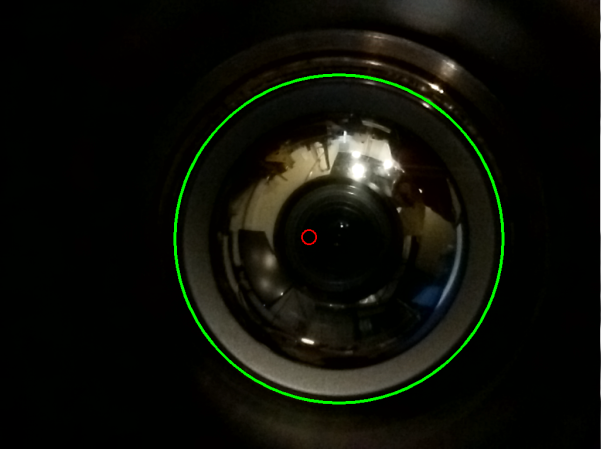
\includegraphics[width=0.7\textwidth]{Centre}
  \caption{\label{fig:centre} The hard-coded centre used for the polar transform
    (red), against the circle detected using the Hough transform (green).
   }
\end{figure}

\textbf{Code Refactor:} As mentioned above, all behavioural code for
the robot has moved into the AntEye application. In fact most code had
been integrated into a single Android Activity (Java Class); this file
contained multiple long threads dictating behaviour as well as a
number of utility methods and robot commands. There were also a large
number of global variables. The resulting file was over 4000 lines
long and almost unusable. Approximately half of the code is useful for
archival purposes only. Consequently, it was decided that it was worth
refactoring the codebase in order to make it easier to work with. All
utility functions were split into their own static Util class,
similarly the robot control commands were moved to the Command
class. Runnable threads were moved into an archive package and split
into classes according to their use: Mushroom Body, Central Complex,
Optical Flow, or Old Navigation; that final group consists of the
oldest code which is not used explicitly but is useful for
reference. A single thread was left in the MainActivity file to act
as a test thread. An amount of unused code was removed entirely.
\newline
\par

Problems remain in the codebase. We identify some such problems and
leave suggestions for further work in our discussion.
\newline\par


\textbf{Video Recording:} In order to analyse the visual processing in
more detail, a video recording utility was added to AntBot. Platform
constraints mean that the utility is not implemented as originally
desiged. A straightforward method using FFMPEG had to be abandoned due
to library conflicts; this method would have allowed a video file to
be recorded directly rather than the frame-stitching solution
described below. The reason this proved difficult was that the
recording had to take place after preprocessing (image unwrapping and
downsampling to the 90x10 $360^{\circ}$ image). In order to achieve
this, frames are passed off to a recording buffer after processing, the
buffer is then processed asynchronously by a separate thread which
saves the frames to a set directory. This does not impact
the frame rate. The video frames are then retrieved from the
robot and stitched together using a custom python utility (a simple
wrapper around an FFMPEG terminal command). The recorded video can then be
analysed offline. This utility was created to allow offline analysis
of optical flow, however it also highlighted a major problem with the
robot which was not previously known; we discuss this next.
\newline
\par

\textbf{Video Pre-processing Pipeline:} When stitching the video
frames from the recorder, we identified that the framerate was not
quite right. The framerate on the robot was found to be an
unacceptably low 2fps which greatly reduced the amount of information
available from the visual system. In an effort to improve the
framerate we isolated different parts of the processing pipeline. We
found the best possible framerate to be approximately 14fps with no
processing (this is computed simply as the number of times the
\textit{onCameraFrame()} callback function is called
per-second). Adding processing steps back to the pipeline, two steps
were found which caused the framerate to degrade. The first step was
an image convolution algorithm; the unwrapped image does not line up
with the direction of travel of the agent, so the resulting frame must
be shifted (azimuth) so that the centre of the frame is in line with
the forward direction. This step was reducing the framerate by
approximately 5fps. Replacing the implemented algorithm with an OpenCV
library implementation reduced the penalty to approximately
1fps. Similarly, an image downsampling algorithm had been manually
implemented which cost around 5fps; replacing this with an OpenCV
library implementation reduced the degradation to approximately
1fps. The full pipeline can now run at 10-12fps with the recording
utility running on top. When simulating a model like the ECX, the
framerate drops marginally to 8-10fps. We also attempted to move the
frame processing into its own high-priority thread, however this
resulted in numerous bugs and did not improve the framerate in any
noticable way.
\newline
\par

 We do not know when the problematic code was added.  In any project
 following its insertion, the framerate surely affected the
 performance of the agent. We can say with certainty that the
 algorithms used and tested in \cite{Mitchell2018} were
 affected. Indeed, in \cite{Mitchell2018} it is noted that few images
 were stored during Visual Navigation experiments. The low storage
 rate was thought to be a thread synchronisation issue, but it is now
 clear that the frames were not finished processing in time to
 be stored.  In testing the matched filter collision avoidance system
 from \cite{Mitchell2018} we note a significant change in behaviour
 after the framerate improvement. It is suspected that this is due to
 an increase in flow information, and therefore an increase in noise
 which can cause erroneous and erratic behaviour, not witnessed in
 \cite{Mitchell2018}.  This is one of the main issues that resulted in
 our lack of results for the ECX.
\newpage

%%%%%%%%%%%%%%%%%%%%%%%%%%%%%%%%%%%%%%%%%%%%%%%%%%%%%%%%%%%%%%%%%%%%%%%%%%%%%%%
% METHODS                                                                     %
%%%%%%%%%%%%%%%%%%%%%%%%%%%%%%%%%%%%%%%%%%%%%%%%%%%%%%%%%%%%%%%%%%%%%%%%%%%%%%%
\section{ Methods } \label{sec:methods}
\subsection{ Collision Avoidance }
% Discuss new method (eight directional FOEs)
Fitting AntBot with sensors which feedback to the higher neural models
is prohibitively difficult (see Discussion). We therefore continue to
look for a method of collision avoidance which can be integrated into
the Central Complex which uses the available visual information. The
matched filter model from \cite{Mitchell2018} performed reasonably
consistently but was initially considered too coarse-grained for
integration into a modified CX. Our first approach therefore looked
for expansion patterns in certain areas of the flow field.

\subsubsection{ Shifting Expansion Fields }
We noted in research that the Focus of Expansion is used in many visual collision
avoidance systems. Usually it is used as a stepping stone to compute the
time-to-contact with an obstacle. Some papers describe using the FOE to determine
a turn direction in the event a collision is detected \cite{Stewart2010,
  Vanderstap2012}. We also note that the often the FOE seems to shift to the
deepest part of the image \cite{Vanderstap2012, Souhila2007} (though we should
also note that in \cite{Stewart2010} an avoidance saccade is triggered
\textit{away from} the FOE); this is not an empirical observation,
however it was enough for us to seek to test if the position of the
FOE was predictable given an approaching scene.
\newline
\par

If the FOE \textit{is} drawn to the deepest part of the image then its
location could be reliably used to choose a steering direction in a
collision avoidance system. Furthermore, this has an intuitive
integration into the CX. If we split the $360^{\circ}$ image seen by
AntBot into eight equal sections reflecting the eight cardinal
directions of the CX model, we can use the horizontal position of the
FOE as an input signal. The position would mark a ``bump'' of activity
in a set of eight neurons (similar to the output layer of the eight
MBON MB model). Ultimately we wish to see if the FOE will behave
predictably in the presence of a looming obstacle, which relies on
being able to compute the FOE reliably.  When working with the FOE,
\cite{Mitchell2018} notes difficulty in computing it
consistently. Often nonsensical values would be output by the
computation. This was suspected to be due to a technical detail not
known at the time of implementation and thus warranted further
investigation\footnote{See \cite{Mitchell2018}, discussion of general
  purpose matrix multiplication in the OpenCV implementation for
  Java.}. Here, we managed to compute reasonably sensible values,
though they were not consistent or predictable (indicating that the
technical problems from \cite{Mitchell2018} did indeed affect the
results). To compute the FOE we use the OpenCV
\textit{calcOpticalFlowFarneback()} function to produce a dense
optical flow field then use the computation from \cite{ODonovan2005}
(see Section \ref{OFBackground}).
\newline
\par

While fixing the problems raised by \cite{Mitchell2018} made the computed FOE
more sensible in terms of general location, the lack of consistency warranted
further investigation. For this purpose, the video recording tool described
in Section \ref{sec:mod} was developed with the goal of performing offline
video analysis of the agent's point of view. Thus, we can visualise the
computed optical flow field observed by the robot under controlled circumstances
(see Figure \ref{fig:flowfield}).\newline\par

\begin{figure}[h!]
  \centering
  
\includegraphics[width=\textwidth]{frame_00066}
  \caption{\label{fig:flowfield} Frame 3 from Figure
    \ref{fig:foeframesempty}. A subset of points from the dense
    optical flow field observed by the agent.  The agent is
    experiencing forward translational motion. These frames were
    captured after the framerate improvement from Section
    \ref{sec:mod}. The FOE is also shown in blue. There are no
    obstacles present in the arena.  }
\end{figure}

This analysis produced the following observations:
\begin{enumerate}
\item{
  The optical flow field is very noisy: The majority of the flow produced
  is erratic and unpredictable.
}

\item{ The amount of perceived motion is exceptionally small: In
  simply looking at the video it is incredibly difficult to determine
  how the motion observed relates to the movement experienced by the
  camera. In most frames the perceived flow is as shown in Figure
  \ref{fig:flowfield}, where each vector is only about 1 pixel in
  length.  }

\item{ The FOE jumps randomly between frames: The FOE is not
  consistent between frames though it can appear to stay in the same
  approximate region (we do not believe this indicates anything
  significant). We cannot rely on its location when presented with a
  looming object in the frame.  }

\item{ Looming objects can be identified from the flow field: This
  observation explains the good performance seen by
  \cite{Mitchell2018} when examining a matched filter system. Looming
  objects can appear as a large (potentially single frame) disturbance
  of the low-level noise produced by the flow field (Figure
  \ref{fig:foeframes}).  }
\end{enumerate}

We can therefore conclude that optical flow cannot be used to compute
any fine-grain properties. The flow field at large is just noise, and
only drastic image changes result in a large disturbance in a specific
region of the flow field. While this effectively precludes any
further investigation into the FOE/depth methods which utilise optical
flow, it does indicate one semi-predictable property of the flow field
which could potentially be used.

\subsubsection{Matched Filters}
The matched filter model of collision avoidance as seen in
\cite{Mitchell2018} was used without modification for the experimental
results in this paper.  However, in an effort to establish the ECX
model, we present here an adaptation of matched filter collision
avoidance which can have its outputs integrated with the CX and MB
models. We will use the language of artificial neural networks, but
the principle is essentially the same as \cite{Mitchell2018}. The
neural approaches presented are all integrated directly into the CX so
that we can make use of the existing architecture and information
available (e.g. the heading information from TB1 and steering output
from CPU1).
\newline\par

The neural model for collision avoidance features two types of neuron, ACC
(ACCumulation) and MRSP (Movement ReSPonse). ACC neurons are key in a working
system, and their representation can affect the behaviour of the model.
\newline\par

\textbf{ACC Neurons:}
ACC neurons take on the role of the leaky accumulators from \cite{Mitchell2018,
  Stewart2010}. The system contains two ACC neurons, ACC$_{left}$ and
ACC$_{right}$ for the left and right sides respectively. We investigate three
different representations of these neurons: Rate, Leaky Integrate \& Fire
(LI\&F), and Reset Integrate \& Fire (RI\&F). The two I\&F variants are only
subtly different and behaved largely the same but we include them for
completeness. We will consider them in chronological order.
\newline\par

The matched filter system produces a sum for the left and right hand sides of the
robot. This sum denotes the difference between the expected motion and the
observed motion in the image frame. If we take the difference between the two
sums we can see if one side has experienced a significant deviation from the
expected motion (i.e. a looming obstacle on that side). This difference acts
as the input to the ACC neurons.
\newline\par

\textbf{ACC Neurons (LI\&F):} For both I\&F models, we need to set a
lower threshold on what we consider an input.  Each input must be greater
than (absolute value) a lower threshold in an attempt to reduce noisy
inputs to the ACC neurons. For more details as to the output from
filter matching, please see \cite{Mitchell2018}. Once the input has
been thresholded, an ACC neuron at time $t$ can be described as:

\begin{equation}
  V(t) = \gamma \cdot V(t-1) + I_{ext}
\end{equation}

where $V(t)$ is the membrane potential, $t$ is the current timestep,
$\gamma$ is the leak current and $I_{ext}$ is the external current
flowing in - the thresholded difference of flow sums.  We use terms
like membrane potential and external current as these best
describe the function in the language of simulated neurons. It should
be noted by the reader that we do not explicitly model voltages and
currents in the model though this is merely a case of semantics; these
properties could be modelled more explicitly.
\newline\par

We also define $V_{fire}$, the value at which the ACC neurons fire.
If $V(t) > V_{fire}$ for some ACC neuron, then the neuron that exceeded
$V_{fire}$ produces an output signal and both have their membrane potential
reset to zero (the resting potential). The neuron that fires then governs the
signal produced by the MRSP layer.
\newline\par

\textbf{ACC Neurons (RI\&F):}
The RI\&F representation is almost identical. The difference arises from the leak
model. In RI\&F we reset the neuron periodically (e.g. every third timestep).
While this is functionally an I\&F neuron, it does not function in any
biologically plausible manner. It is essentially the same as the leaky
accumulators from \cite{Mitchell2018}. We can describe the RI\&F neuron at time
$t$ by:

\begin{equation}
  V(t) =
  \begin{cases}
    V(t-1) + I_{ext} & \text{if } t \not\equiv 0 \bmod p \\
    0 & \text{otherwise}
  \end{cases}
\end{equation}

where $V(t)$, $I_{ext}$, and $t$ are as above and $p$ is the reset period (for
example, if $p = 3$ the membrane potential is reset every 3 timesteps). Firing
behaviour is the same as the LI\&F model.
\newline\par

\textbf{ACC Neurons (Rate):}
While I\&F neurons provide an intuitive neural metaphor for the leaky
accumulators, the CX model (into which this CA system is being built) uses
a rate model for all other neurons (including our own MRSP neurons). As such we
felt it appropriate to investigate such a representation for the ACC layer. In
fact, using a rate representation requires only a single ACC neuron and allows
for the generation of a steering response which is proportional to the size of
the optical flow disturbance (in theory, the bigger the obstacle or loom effect,
the bigger the response); neither of which are possible with the I\&F
representation. Recall, a firing rate given some input $I$ is represented as a
sigmoid (Eq. \ref{eq:sig}):

\begin{equation*}
r = \frac{1}{1 + e^{-(aI - b)}}
\end{equation*}

where $a$ and $b$ determine the \textit{slope} and \textit{bias} of
the function respectively. If we set $a = 5$, $b = 0$ we obtain the
rate function shown in Figure \ref{fig:accrate}. Importantly, we must
scale down the input (difference of flow sums) such that it lies in
(-1,1).\newline\par

\begin{figure}[h!]
  \centering
  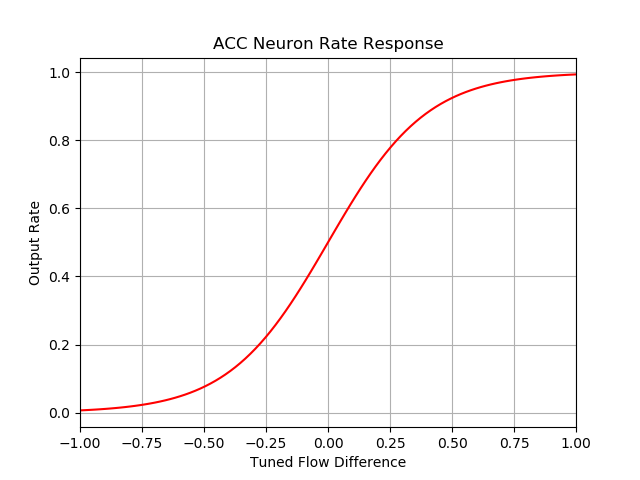
\includegraphics[width=0.9\textwidth]{ACCRate}
  \caption{\label{fig:accrate} Function of firing rate response of the single ACC
    neuron against difference input; sigmoid with $a = 5$, $b = 0$. The input to
  this neuron is scaled down to lie between -1 and 1.}
\end{figure}

If the flow disturbance observed on both sides is equal, then the rate
response should lie around 0.5. A looming object detected on the
right-hand side results in a negative input drawing the output closer
to 0. Conversly, a looming object detected on the left-hand side will
result in a positive input, driving the output closer to 1. We have,
in a roundabout way, ended up with an optical-flow balance strategy -
a flawed, simplistic, yet not entirely implausible hypothesis for
collision avoidance in insects \cite{Julien2017}. If our output
remains close to 0.5 we need not react, close to 1 we must turn right,
and close to 0 we must turn left. Thus, with a single neuron we can
react to both scenarios; furthermore, the signal is proportional to
the disturbance observed and we can therefore scale our steering
command as necessary. This method is simple and flexible, though it is
highly susceptible to noise, as we will see this is a critical flaw.
\newline\par

\textbf{MRSP Neurons}: There are 16 MRSP neurons laid out in the same
fashion as the CPU4 layer. The MRSP connects to CPU1 using the same
connection pattern as CPU4-CPU1 in the existing CX model. For clarity,
the MRSP neurons always use a rate representation. In all cases the
MRSP layer functions by generating a sine wave with the peak in the
desired direction of travel; the method for constructing and
positioning this sine wave is purely algorithmic, we did not
investigate a way to model this behaviour using neural connections.
\newline\par

We first create an array of eight evenly distributed points on a
shifted sine wave.  The curve is shifted by $-\frac{\pi}{2}$ in the
$x$-axis such that $\sin(\frac{\pi}{2})$ is in the first element (this
is simply housekeeping, it makes index arithmetic easier when creating
the output). The peak of this sinusoid array will denote the desired
direction of travel, we therefore need to shift the array so that the
maximum lies in the correct place. This \textit{shift} is calculated
as $\textit{shift} = \textit{current\textunderscore direction} +
\textit{offset}$. The current direction can be read from the TB1 layer
(the TB1 neuron with the highest firing rate). The offset is computed
based on the response from the ACC layer; this computation is
different in the I\&F and Rate cases.
\newline\par

In the I\&F case, the offset will be -2, 0, or 2 depending on which
ACC neuron fires (ACC$_{right}$, both/neither, or ACC$_{left}$
respectively). This is a coarse but functional reaction which
generates a saccade of approximately $30^{\circ}$ in either
direction. We included the case where both fire to act as a balance
case, however, in practice this never happens. This is functionally
identical to the behaviour displayed by the CA system in
\cite{Mitchell2018}, piped through the CX structure.
\newline\par

In the Rate case, we instead receive a single input from the ACC layer.
This input will lie in (0,1) and we need only a simple linear transform to
choose an offset from this value. The transform has the conditions that
$f(0.5) = 0$, $f(1) = 2$, and $f(0) = -2$.

\begin{equation}
  \label{eq:transform}
 f(x) = 4x - 2
\end{equation}

satisfies these conditions. The output of Eq. \ref{eq:transform} is
then rounded to the nearest integer to determine the offset.  \newline\par

In both cases, once the offset has been determined the sinusoid array
will be shifted such that the maximum is in the desired element. The
shifted sinusoid array is then extended to sixteen elements to match
the CPU4 representation. The final extended sinusoid array is used as
input to the MRSP neurons whose output is computed as:

\begin{equation}
  \label{eq:rmrsp}
  r_{MRSP} = \frac{1}{1 + e^{-(5I - 2.5)}}
\end{equation}

The computed firing rates are then supplied to the CPU1 layer of the
CX by utilising CPU4-CPU1 connection array. The CPU1 layer then
generates the steering command. In fact, as the MRSP layer utilises
the same neural architecture as CPU4, we can give the input to CPU1
as:

\begin{equation}
I_{CPU1}^{(t)} = r_{MRSP}^{(t)} - r_{TB1}^{(t)}
\end{equation}

Note that this is in the case where we only the CA system is
contributing to the output (i.e. no path integration or visual
navigation). The TB1 subtraction is still required in the input to
generate an avoidance saccade relative to the current heading of the
agent.
\newline\par

An example of the signal propogation from ACC (rate-based) response to
MRSP output can be seen in Figure \ref{fig:mrspRateResponse}. Input
($I=0.25$) is supplied to the ACC neuron, its firing rate ($r=0.78$)
is put through the offset computation function ($\textit{offset} =
1.11 \rightarrow 1$), and this offset is added to the current
direction ($\textit{current\textunderscore direction} = 4$ in the
example) to give the total offset. The sinusoid array is rotated such
that the maximum (index 5) indicates the desired direction of travel,
the sinusoid is extended to sixteen elements and supplied as input to
the MRSP neurons; the MRSP firing rate is given by Eq. \ref{eq:rmrsp},
and an example MRSP layer output is shown in Figure
\ref{fig:mrspRateResponse}.

\begin{figure}[h!]
  \caption{\label{fig:mrspRateArrangement}[PLACEHOLDER] \textit{This
      figure will show the full architecture of the rate-based system.}}
\end{figure}

\begin{figure}[h!]
  \centering
  \vspace{-45pt}
  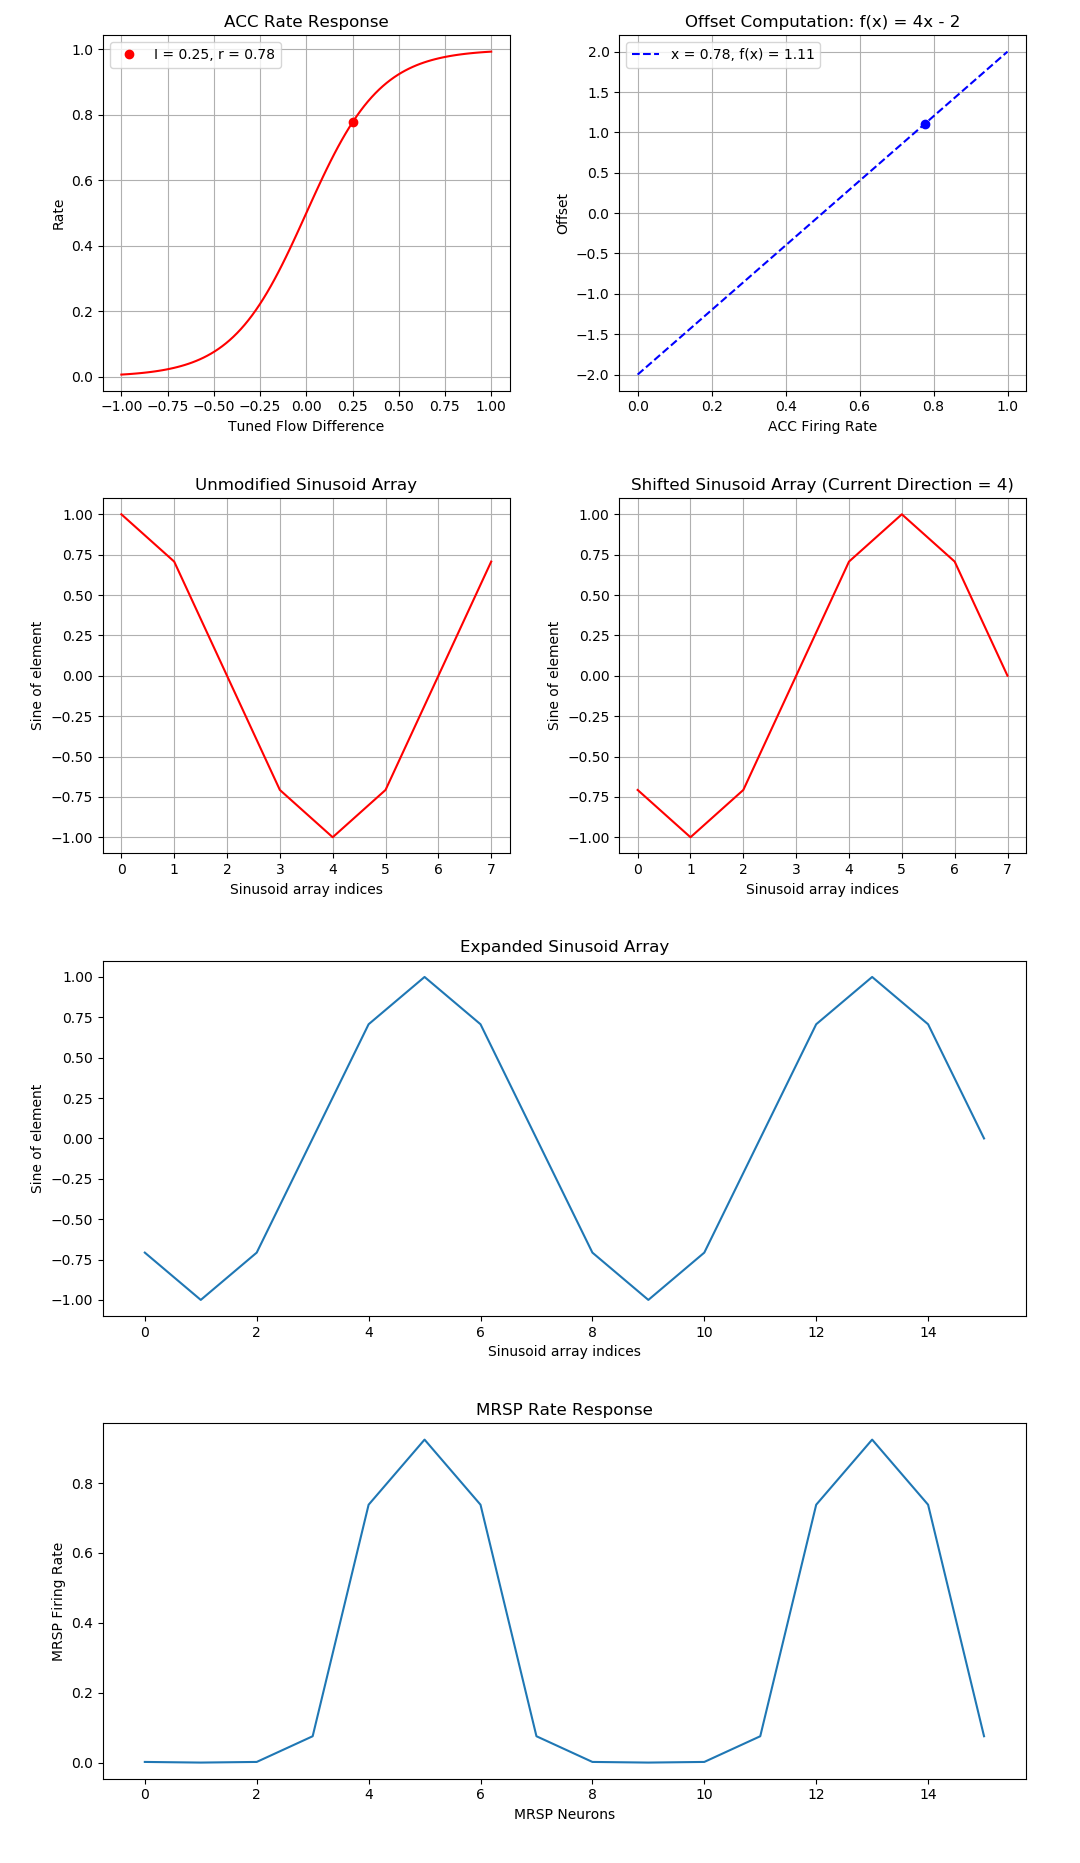
\includegraphics[width=0.8\textwidth]{NeuralCASignalProp}
  \caption{\label{fig:mrspRateResponse} An example of signal
    propogation and generated output from the rate-based system
    (left-to-right, top-to-bottom). An example flow input is given as
    0.25. The ACC rate response is then put through the offset
    computation function (Eq. \ref{eq:transform}). The default
    sinusoid function is generated over eight array elements. The
    sinusoid is then shifted such that the maximum lies at
    \textit{current\textunderscore direction + round(offset)} which in
    this case is 5. This sinusoid is then extended to a sixteen
    elements to match the representation in CPU4. Each element of the
    sinusoid is then supplied as input to the corresponding MRSP
    neuron to give the rate output in the final plot; as there are two
    neurons for each cardinal direction, the two maxima indicate a
    single direction. This MRSP response is used as input to the CPU1
    layer, in this example a small right turn will be generated.  }
\end{figure}


\subsection{ Path Integration }
The path integration circuit in use is a slightly simplified version of that
presented in Section \ref{CXBackground}. This version does not model the
TN neurons or the Pontine neurons. The model is the same as that used in
\cite{Scimeca2017, Zhang2017}, and the robot-based tests from \cite{Stone2017}.
\newline\par

We use the CX firstly for a round of experiments in which we wish to address a
key methodological flaw observed in the experiments of \textit{Zhang}
\cite{Zhang2017}. We then use the CXMB variant (the 8-MBON model)
as the basis for the ECX model. \textit{Zhang} does not make it entirely clear
(though it is stated) that the 8-MBON model is actually an adapted CX model.
Distance measurements are arbitrary, there is no access to wheel encoder
measurements. Unlike previous works, the agent moves only in the forward
direction so we can reasonably assume that the robot will travel roughly the same
distance in a set time interval.

\subsection{ The Complete System}
A complete model has been constructed. Present on the robot is a
singular model which, in theory, will perform collision avoidance,
path integration, and direction-associated visual memory
(simultaneously); however, we did not manage to collect formal results
due to technical and time constraints (though some informal testing
has been conducted). We present the model here and present the issues
experienced and learning points in Section \ref{sec:results}.
\newline\par

In an effort to keep the integration simple, first version of this
model allowed the collision avoidance system to fully overwrite any
steering instruction in the event of a detected obstacle. While
straightforward and intuitive, this method proved too coarse. If a
full model was to be constructed, it was clear that a full neural
representation for the collision avoidance system would need to be
constructed; this and tested variants have been described above.
\newline\par

The final model takes the 8-MBON CXMB model and inserts the additional ACC and
MRSP neurons required for the integrated collision avoidance system. The
connections between TB1 and MRSP are the same as the connections between TB1
and CPU4, likewise the connections between MRSP and CPU1 are the same as those
between CPU4 and CPU1. In fact, as the eight MBONs are expanded out to a
sixteen neuron representation (see Section \ref{CXMBBackground}) the
model can be visualised as the CX with two additional layers of sixteen neurons
between CPU4 and CPU1 plus one or two ACC neurons depending on the neural
representation used. The final version implemented on the robot used the rate
representation for a single ACC neuron.
\newline\par

The output of the network can be selected by changing the mode of the
CPU1 output stage. In this fashion, one can isolate each system and produce
the steering output using specific systems. The key modes currently present on
the agent are CA-only, and CXCA which are the isolated collision avoidance system
and the combined output of the path integrator and the collision avoidance
system respectively; adding further combinations should be trivial. The
selection currently available is due to the component level testing that
was in progress towards the end of the project. The weighting applied to each
layer can be specified and ideally it should be dynamic. While the visual
memory infrastructure is entirely present, it was not tested; however, as stated,
it is identical to that presented by \textit{Zhang} so we have no reason to
think that this subsystem should not work to the degree presented in
\cite{Zhang2017}.

\begin{figure}
\caption{\label{fig:ecx} [PLACEHOLDER] Attempt to show the full thing if possible
  but this may be prohibitively difficult.}
\end{figure}

\subsection{Tussocks}
During \cite{Mitchell2018}, we note that the tussocks were extremely
small in the view of AntBot; furthermore they were incredibly
fragile. They were originally constructed by connecting synthetic
boxwood bushes to wooden blocks with wood glue; the glue became
disconnected quickly and all had to be repaired with superglue
multiple times during the experimentation phase of
\cite{Mitchell2018}. For convenience, we construct new synthetic
tussocks. The basic idea is the same, but the wood blocks were made
larger, and the synthetic foliage sits higher. The two pieces were
stapled together resulting in a much more robust structure. From video
data it can be seen that they are far more prominent in the image
frame, as required.

\section{Experimentation and Testing}\label{sec:test}
We re-use the experimental environment from \cite{Mitchell2018}. A
collapsible boundary wall is constructed on the robot-football pitch
in room G.17 in the Informatics Forum. Small ``tussocks'' are used as
objects in the environment (e.g. to avoid or to provide visual
information). A sequence of VICON motion-capture cameras are arranged
in a ring above the pitch and allow accurate tracking of the agent's
movement and heading.

\subsection{Path Integration}
The first round of tests aims to establish firmly that the CX model is capable of
robust path integration in the real world. The CX has undergone reasonably
extensive testing on the AntBot, however, two key issues were noted across all
tests.

\begin{enumerate}
\item{ The outbound route of the agent is always the same. While this
  route was randomly chosen, it was the same in all trials. It is
  entirely possible that any parameter tuning was performed with
  respect to this route. Good performance on a single route does not
  indicate good performance as a general path integrator.  }

\item{
  The outbound route always finishes with the agent directed at the nest. This
  means that the robot could potentially navigate home by making little to no
  change in its trajectory.
}
\end{enumerate}

The second problem is more of a symptom of the first; to remedy both problems we
need only fix the first. This can be done in a few ways. Firstly, we could
simply generate a randomised turning command at set (or even random) intervals.
There are many variations on this theme, however the original goal of this paper
was to provide a complete navigational system. It makes more sense for us to use
a collision avoidance system to generate the outbound routes.
\newline\par

We use the collision avoidance system from \cite{Mitchell2018} to fill this
role. For the standard CX experiments, this collision avoidance system was
entirely unmodified and separate from the path integration circuit. The outbound
route was governed by the CA system (with the path integrator updated on each
step) and the inbound route was governed entirely by the CX. These experiments
pre-date the neural collision avoidance system so there is no way to provide
CA and PI behaviour simulaneously. Thus, the experimental arena was carefully
chosen based on known properties of the CA system.
\newline
\par

For half of the runs the agent was started from the tape markings in
the South West corner of the arena and for the other half the agent
was started from the marking at the South end.  We place only two
tussocks in the South East corner of the arena to ensure the agent is
always directed into the arena. The full reasoning behind this
obstacle placement is given in \cite{Mitchell2018}; while navigation
towards the arena wall is still successful CA behaviour, it is not
useful for testing higher navigational systems. The rest of the arena
is left clear. The CA system from \cite{Mitchell2018} is sensitive
enough to provide non-deterministic reactions where no direct
obstacles are present whilst successfully avoiding the arena walls
(see CA experimental results from \cite{Mitchell2018}). We therefore
manage a non-deterministic outbound route based on CA while keeping
the arena clear for the PI stage of the test. These experiments were
conducted before the framerate improvement so CA behaviour can be
considered comparable to \cite{Mitchell2018}. Any test in which the CA
system failed catastrophically (direct collision) was to be ignored as
only the CX was to be tested, though there was only one such case.
\newline\par

The agent was permitted to make a $180^{\circ}$ (approx.) turn at the
end of the outbound route. In most cases, this does not make the robot
point directly towards the nest. The justification for this procedure
can be seen in Figure \ref{fig:cxnt}. The output from the CX model is
a left/right turning instruction with some strength; the greater then
angle between the current and home vector, the greater the output
signal in the required direction, however, the output is not the
precise angular correction required. As such, the agent required a large
turning arc (and a long time) to reorient itself with the home vector
before it could even begin the journey. Encouraging as this behaviour
is for the performance of the CX circuit, we felt it more practical to
avoid it for formal experiments as most outbound routes did not leave
enough space for these arcs.
\newline\par

\begin{figure}[h!]
  \centering
  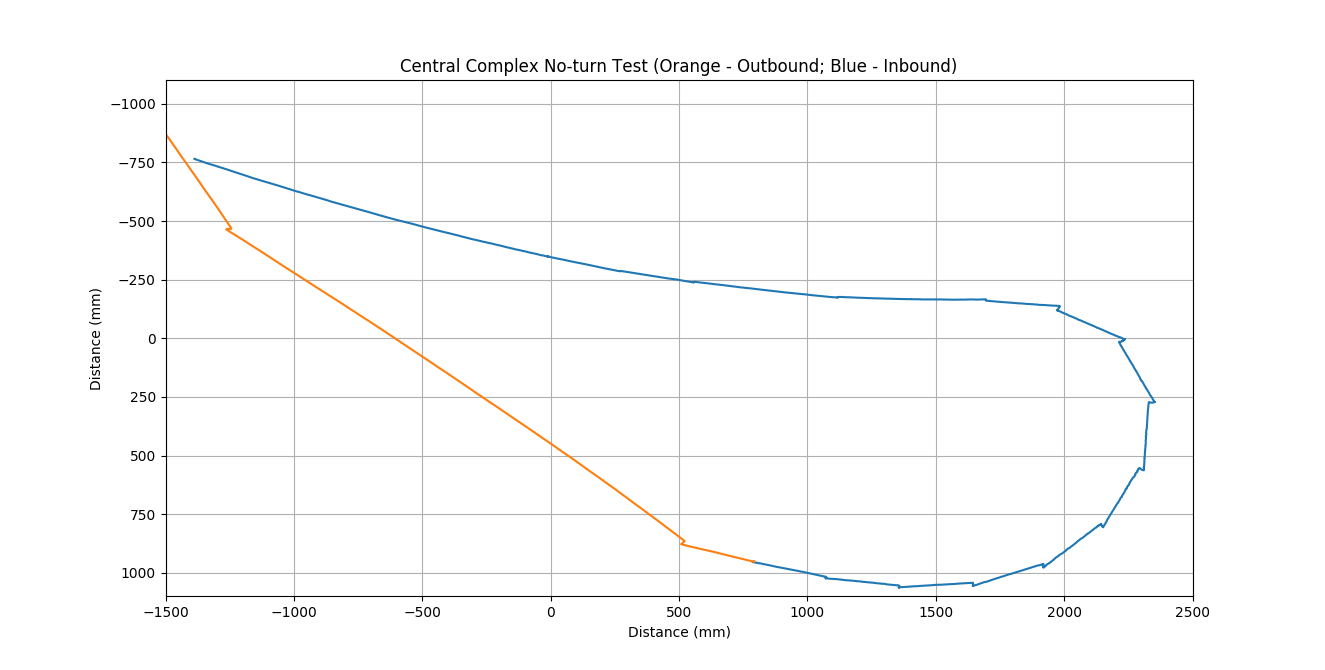
\includegraphics[width=\textwidth]{CXNT}
  \caption{\label{fig:cxnt} A test recording from the Central Complex
    PI experiments. The agent successfully navigates home but requires a large
    turning arc to point back towards the nest. This is because the output of the
    CX is not a precise angle but instead a turn direction with some strength.
    This behaviour was our prompt and justification to include an about turn on
    completion of the outbound route; the space present in the arena simply did
    not permit such routes for formal experiments.
  }
\end{figure}

Success was measured by the ability of the agent to touch the tape
square from which it started. This could be any part of the robot
(e.g. a tread running over the corner of the square). The agent was
stopped manually once either a success state was reached or a success
state could not be reached; for example, if the robot collided with
the arena wall during PI, or passed the start point without touching it.
\newline\par

Finally,  we should note that the locomotion of the robot is different to that of
previous tests. Previous works with the CX model look to keep the motion of the
agent continuous. The impracticality of such motion on the AntBot is noted in
\cite{Mitchell2018} and below in our own discussion. Instead, we keep the motion
in discrete steps; the agent moves forward, stops, turns on the spot, and
continues. In the case of the PI experiments, the oubound route is made up of
steps broken by turns generated from OFCA at irregular intervals, the inbound
route consists of steps broken by regular course correction turns (e.g. every two
seconds, the CX output is checked); this behaviour can be seen 
clearly in Figure \ref{fig:cxnt}. The distance measurement is still updated
continuously; we use time-travelled as the distance metric (assuming we
travel the same distance in the same amount of time). While this is generally
considered a poorer way to measure distance, many problems are mitigated by the
fact the agent only moves in the forward direction, and to a degree this model
should be robust to \textit{rough} or \textit{noisy} inputs. We are pleased to
report that the CX performs well, even with a problematic distance metric.

\subsection{Collision Avoidance}
\subsubsection{Shifting Expansion Patterns}
The initial tests for the shifted expansion pattern system involved computing
a FOE and checking for its horizontal position in the image frame. Our
original hypothesis was that the FOE would be drawn
to the deepest part (frontal) of an image, and therefore its horizontal position
would dictate the desired direction of travel. We would, of course, take any
predictable behaviour which could be used for collision avoidance.
\newline\par

The agent was set on a collision course with a cluster of tussocks and
watched for consistent reaction behaviour. No consistent behaviour was
observed.  To test our hypothesis completely, it was clear that
further work was needed to verify that there was no usable
behaviour. The processed image frame (the view of the agent) can be
viewed on the smartphone screen; the view is too small to pick out any
details of a flow-vector field. As a general point, testing optical
flow behaviour on the robot is quite difficult due to the field of
view. Even outputting an FOE location and moving an object in front of
the robot cannot tell us if we are producing the desired behaviour;
firstly, because the object will not move realistically in the frame;
and secondly, because the robot will observe motion from all
directions (due to the 360$^\circ$ view) which would not normally be
present; for example, the body and arms of the tester manipulating the
object will not match the pattern of motion which would be observed
during locomotion, thus affecting the output. This is true for all
visual testing with the robot; it is hard to produce reliable output
as the input is likely unrealistic.
\newline\par

Two solutions to this problem have been developed over previous years:
\textit{LogToFileUtils} developed by \textit{Zhang} to provide textual
logging utilities where it was not normally possible to use such logs
\cite{Zhang2017} and \textit{StatFileUtils}, a variant of
\textit{Zhang's} logging utility which produced regular file output
which could be easily parsed to produce graphical plots from recorded
data \cite{Mitchell2018}. Neither were useful in testing the FOE
position; we could log it, but there was be no way of correlating its
behaviour with the agent's view of the environment. Instead, we chose
to implement a video recording tool which would allow us to record
controlled runs of the agent through an environment. Furthermore, this
video could be processed offline using the same systems implemented on
the robot, then scaled up to give a much clearer view of what the
robot was actually seeing.  This proved incredibly useful and allowed
us to immediately dismiss shifting expansion patterns as a method for
collision avoidance on the AntBot.
\newline\par

The recording tool was used to show the infeasibility of this method
informally, however, we present below some frames from formal
recordings, taken to demonstrate our findings for the purpose of this
paper. Two such recordings were taken, both in the experimental
arena. The first was taken with no objects present, and in the second, the
arena contained two objects staggered to the right and left of the
robot's path. These objects were not in the robot's direct path.
In both recordings the direction of motion was entirely
translational in the direction of view; no turns took place. The robot
was permitted to move from one end of the arena to the other without
interruption, aside from a manual stop which was done with minimal
disturbance. The arena can be seen in Figure \ref{fig:foetest}, the
robot's intended path is shown in red.

\begin{figure}[h!]
  \centering
  \includegraphics[width=\textwidth]{FOETest}
  \caption{\label{fig:foetest} The non-empty arena used for testing
    the shifting expansion field system. Tussocks were set to the left
    and right of the robot's trajectory (shown in red) so that they
    were not on a collision course but should still affect the
    expansion field. We had hoped the FOE would either remain central
    or drift horizontally (in a consistent fashion) as each object was
    passed. Note that the agent was not started directly on the tape
    square, it was offset as shown by the path; this was oversight on
    our part.  }
\end{figure}

\subsubsection{Neural Matched Filters}
The testing for the neural matched filter system was far more
simple. In this case, we know that the underlying method (matched
filter collision avoidance) is sound, we just wish to translate it
into a neural representation. Thus, the first thing we need to test is
the ability to generate an arbitrary turn by inducing activity in the
MRSP layer of the model. We take the current direction from the TB1
layer, generate our sinusoid array and shift it to the left or right of the
current heading. We can then check if we can generate consistent
steering commands.
\newline
\par

We then test the three different implementations of the ACC neurons
separately. Each type was tested initially in an empty arena. This
basic test ensured that reactions were being generated and that the
system was responding in a sensible, sensitive fashion. We then add an
obstacle.  For each ACC implementation, the agent was started in the South
end of the arena, on a collision course with a cluster of tussocks
positioned in the centre. We wished to see if the neural system would
replicate the performance of the neural matched filter system from
\cite{Mitchell2018} by starting with a variation of the most basic
obstacle avoidance scenario presented (Table 2, Arena 2 from
\cite{Mitchell2018}).
\newline\par

No system performed consistently well in the presence of an obstacle,
however the I\&F variant\footnote{As behaviour between the two I\&F
  variants was identical, we will discuss them together going
  forward. Most testing took place with lI\&F ACC neurons.} provided
sufficiently consistent reactions to observe some runs of the
ECX.

\subsection{ECX (CXCA)}
The testing methodology for the ECX was to test each individual system
and then the full combination. There is a set order to this testing as
each step of the integration requires some prerequisite (except
CA). The CA system must be tested first, then the combination of CA
and PI (CACX) as we need working PI to learn homeward visual routes,
finally, the MB can be connected and the full ECX can then be tested.
\newline\par

All systems are implemented and available; we present testing only up
to the CACX implementation. The CACX was tested (informally) by
allowing the combined system to navigate homeward following a
successful collision free outbound run. The combined model was
only tested using the I\&F variant of the neural CA model as this
version managed successful collision avoidance behaviour. As CXCA
tests followed successful CA tests, the CXCA is tested in the same
environments: an empty environment and one with a single large
cluster of tussocks.


\section{ Results } \label{sec:results}
\subsection{ Path Integration }
We are pleased to report good performance from the CX model. We
observed successful homing in 7/10 tests performed, though in all
cases the agent proceeded in the correct general direction. Of the
failures, two were minor and one was more significant. The full
results can be seen in Table \ref{tab:cxres}.
\newline
\par

\begin{table}[h!]
  \centering
\begin{tabular}{|c|l|l|l|}
\hline
\multicolumn{1}{|l|}{\textbf{Test}} & \textbf{Start Point} &
\textbf{Success/Failure} & \textbf{Distance from Start Point (mm)} \\ \hline
\textbf{AB\textunderscore CX\textunderscore 1}                          & SW                   & Success                  &  306                                  \\ \hline
\textbf{AB\textunderscore CX\textunderscore 2}                          & SW                   & Success                  &  348                                  \\ \hline
\textbf{AB\textunderscore CX\textunderscore 3}                          & SW                   & Failure                  &  517                                  \\ \hline
\textbf{AB\textunderscore CX\textunderscore 4}                          & SW                   & Success*                 &  325                                  \\ \hline
\textbf{AB\textunderscore CX\textunderscore 5}                          & SW                   & Failure                  &  581                                  \\ \hline
\textbf{AB\textunderscore CX\textunderscore 6}                          & S                    & Success                  &  356                                  \\ \hline
\textbf{AB\textunderscore CX\textunderscore 7}                          & S                    & Success                  &  304                                  \\ \hline
\textbf{AB\textunderscore CX\textunderscore 8}                          & S                    & Success                  &  296                                  \\ \hline
\textbf{AB\textunderscore CX\textunderscore 9}                          & S                    & Success                  &  311                                  \\ \hline
\textbf{AB\textunderscore CX\textunderscore 10}                         & S                    & Failure**                & 458                                   \\ \hline
\end{tabular}

\caption{\label{tab:cxres} The compiled results from the CX path
  integration experiments. (*) While this test succeeded, it was
  close.  The CA system failed at the last section of the outbound run
  which could be the cause of the near-failure. (**) We consider this
  the worst failure; while this run is not the furthest from its start
  point, it can be seen from Figure \ref{fig:abcx10i} that the agent
  actively deviates from its route.  }

\end{table}

VICON recordings from all tests are available in Appendix
\ref{ap:cxfigs}. While the results appeared good under observation and
in the figures, we must note the distance measurements in Table
\ref{tab:cxres}. These measurements are taken from the central axis of
the VICON skeleton applied to the robot, approximately the central axis
of the robot. Due to the size of the robot, we must note that our
success criterion may be deceptive. The closest arrival at the nest is
29.6cm; while the robot did indeed make it back to its starting box,
this is still a reasonably large deviation. Given that the agent's
general direction is almost always correct (except Figure
\ref{fig:abcx10i}), we think it is reasonable to presume that the deviation
could be due to the inaccurate odometry; counting timesteps where an
agent is in motion is generally considered a crude and inaccurate
method of tracking distance travelled, we use this method as it was
all that was immediately available on the robot (see Discussion).
\newline\par

\begin{figure}[h!]
  \centering
  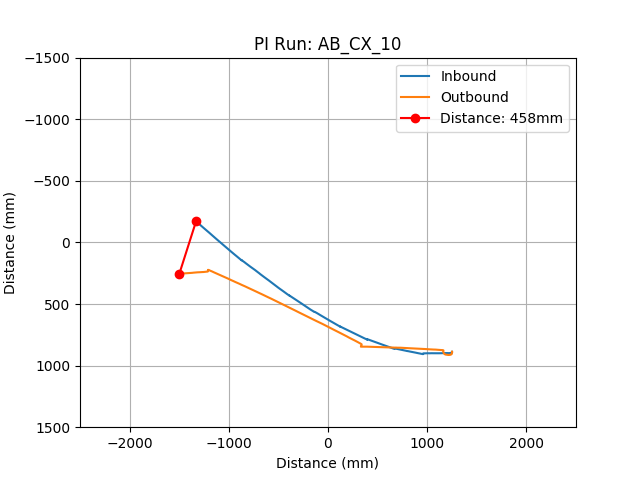
\includegraphics[width=0.8\textwidth]{AB_CX_10}
  \caption{\label{fig:abcx10i} PI test AB\textunderscore
    CX\textunderscore 10. This was considered the worst failure of the
  system despite not having the greatest deviation from the start point.}
\end{figure}

An example of favourable behaviour (under experimental protocol) can
be seen in Figure \ref{fig:abcx8i}. In this case, the agent is already
close to its home vector but still corrects to achieve more accurate
homing. This is also the run which achieves the best performance by
the distance-to-start measurement.
\newline\par

\begin{figure}[h!]
  \centering
  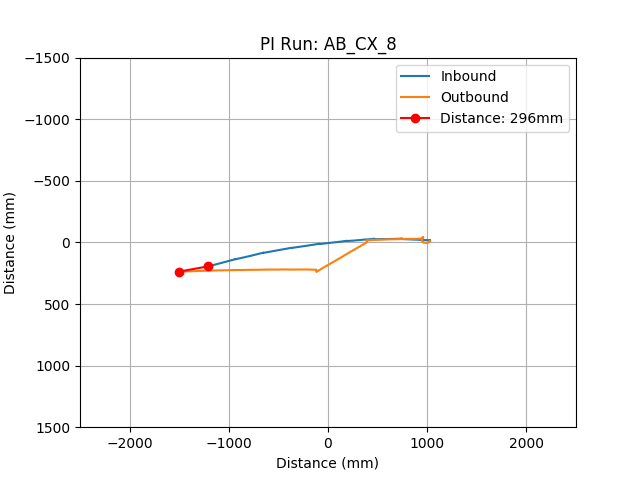
\includegraphics[width=0.8\textwidth]{AB_CX_8}
  \caption{\label{fig:abcx8i} PI test AB\textunderscore
    CX\textunderscore 8. Arguably the most successful recording from
    the formal experiments. The agent still corrects to achieve a
    better homing path, despite the fact it could likely have
    travelled in a straight line. }
\end{figure}

While we still consider these experiments to be a successful
demonstration of the capability of the CX (especially with the early
test run in Figure \ref{fig:cxnt}), we must acknowledge certain
methodological issues. Firstly the deviation and secondly the run
length. All runs can be seen to be very short. We think it would be
prudent to repeat these experiments with longer runs and more accurate
odometry (see Discussion). Despite our justification, it may also be
prudent to remove the 180$^{\circ}$ turn at the end of the outbound
run; perhaps 90$^\circ$ would allow the network to perform corrections
while still removing the need for large loops. In some recordings, it
can be seen that the robot is still pointing directly home after its
outbound run (Figure \ref{fig:abcx1i}), though this is not always the
case.

\begin{figure}[h!]
  \centering
  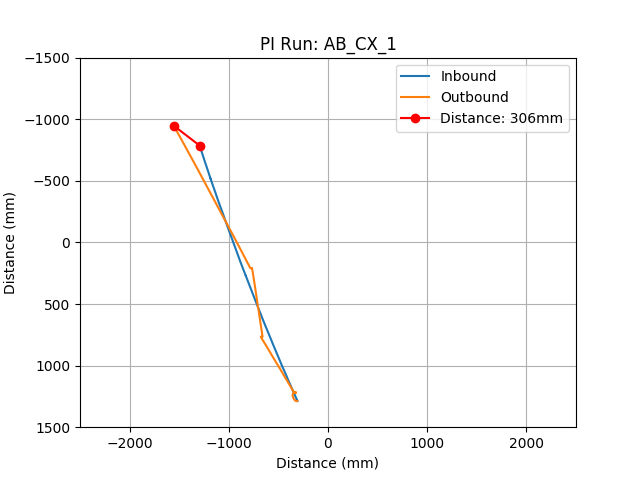
\includegraphics[width=0.8\textwidth]{AB_CX_1}
  \caption{\label{fig:abcx1i} PI test AB\textunderscore
    CX\textunderscore 1. In this case, we note the exact same
    experimental flaw we sought to avoid in which the robot requires
    no correction to home successfully.}
\end{figure}

\subsection{Collision Avoidance}
\subsubsection{Shifting Expansion Patterns}
The optical flow experiments conducted allow us to state with a high
degree of confidence that the FOE cannot reliably be used as the means
to generate a steering command in the case of the AntBot. We limit our
conclusions to the AntBot as:

\begin{enumerate}
\item{This is the only platform on which we have tested the predictability
  of the FOE.}

\item{ The works which inspired this method achieved success in using
  the FOE to direct motion \cite{Stewart2010, Vanderstap2012}.}
\end{enumerate}

Therefore, we conclude that it is likely that the AntBot's unique
360$^\circ$ field of view and low resolution vision play a major role
in the problems experienced. For an example, consider the five image
frames presented in Figure \ref{fig:foeframes}.
\newline\par

\begin{figure}[h!]
  \centering
  
\includegraphics[width=\textwidth]{frame_00057}
  
\includegraphics[width=\textwidth]{frame_00058}
  
\includegraphics[width=\textwidth]{frame_00059}
  
\includegraphics[width=\textwidth]{frame_00060}
  
\includegraphics[width=\textwidth]{frame_00061}
  \caption{\label{fig:foeframes} Five consecutive image frames with
    optical flow information superimposed over the top. It can be seen
    that the FOE position (central pixel of the blue cross) is not
    consistent across multiple frames. This figure also shows the
    disturbance caused by approaching a tussock on the right hand side
    (3rd and 4th frames). Video captured at approximately 10fps
    (i.e. these images were captured accross roughly 0.5 seconds).
  }
\end{figure}

These five frames show how the FOE tracks across the azimuth in the
course of approximately half a second. This certainly allows us to say
that the FOE is not drawn to the deepest part of the image frame,
which should be centre to centre-left across all five frames. These
frames would also indicate that the FOE position is not predictable
given the motion experienced - it is in fact more accurate to say, the
fine motion perceived is not predictable. To show this more concretely
we can look to another example in Figure \ref{fig:foeframesempty}.
\newline\par

\begin{figure}[h!]
  \centering
  
\includegraphics[width=\textwidth]{frame_00064}
  
\includegraphics[width=\textwidth]{frame_00065}
  
\includegraphics[width=\textwidth]{frame_00066}
  
\includegraphics[width=\textwidth]{frame_00067}
  
\includegraphics[width=\textwidth]{frame_00068}
  \caption{\label{fig:foeframesempty} Another set of consecutive
    frames, this time captured in an environment with no objects
    present. The FOE is still unpredictable, though it does not move
    as drastically in the horizontal axis.
  }
\end{figure}

In this case there are no obstacles present in the arena, and thus
there should be minimal sources flow field disturbance. Nevertheless,
we can still see that the FOE jumps, though not quite as drastically.
The views are perhaps deceptive due to the pre-processing but for
clarity we note that each pixel represents 4$^\circ$ of horizontal
arc. Even small FOE jumps in the image frame are large with respect to
the world.\newline\par

While it would be interesting to test empirically such use of the FOE
in a different setting, we can conclude that the FOE may not be used
to govern any control output on the AntBot; indeed, we would go so far
as to conclude that the FOE is of no use to the AntBot at all.
\newline\par

The remainder of our results discussion arises from developmental testing.
These are not results from which concrete conclusions may
be drawn, however they may provide insight for anyone considering
implementing the neural filter model for collision avoidance, or the
ECX, as a continuation of this work.

\subsubsection{Neural Matched Filters}
The three variants of the neural filter model involve using the
different representations of the ACC neurons. In testing, the I\&F
versions performed identically under observation, so we will discuss
them as one.\newline\par

\textbf{I\&F:} Performance of the system was promising though
inconsistent, however collision free behaviour was observed. Behaviour
was similar to, though not as consistent as, that observed in
\cite{Mitchell2018}.
\newline\par

In the obstacle free case, the system mostly managed to avoid the
arena walls. The behaviour seemed more sensitive than
that given by \cite{Mitchell2018}. The algorithmic matched
filter system also experienced problems in an empty arena, so similar
behaviour in the neural model did not prove discouraging.
\newline\par

With an obstacle present, the behaviour of the system was initially
positive. The agent did in fact manage to navigate around a single
large obstacle successfully on multiple ocassions. However, the
behaviour was inconsistent; in many cases the agent would turn towards
the obstacle coming very close to collision (or actually colliding)
with the obstacle. On some occassions the agent would avoid the
obstacle and then collide with the arena wall. Performance here was
positive enough to warrant testing with a sparsely occupied
environment (two tussocks per pitch quadrant); at this point the
observed performance broke down, collisions became far more common
with many being caused by unnecessary turns \textit{towards} obstacles
(i.e. the agent's path was clear but a turn was triggered, often
putting the agent at immediate risk of a collision). The architecture
is clearly functioning as intended, however, further tuning of the
input is required to obtain consistent collision avoidance behaviour
(see Section \ref{sec:future}).
\newline\par

%% Unfortunately, the performance was generally poor,
%% though this was the only variant which managed successful collision
%% free runs (not consistent enough to gather any formal
%% data). It is no surprise that this variant came closest to replicating
%% the behaviour (if not the performance) of the original model from
%% \cite{Mitchell2018} as it is, functionally, a dressed up version of
%% this model (with the addition of neural steering generation).
%% \newline\par

%% With this in mind, one could reasonably ask why this model does not
%% function consistently where the one from \cite{Mitchell2018}
%% did. Indeed, we used the model from \cite{Mitchell2018} successfully
%% in this work for our path integration experiments (and it was tested
%% successfully alongside the MB model in a cluttered environment during
%% the code refactor process). The neural OFCA model was implemented
%% after the improvements to the visual pipeline; as this was the only
%% change, we suspect this is the problem. In testing the original
%% model from \cite{Mitchell2018} \textit{after} the improvement to the
%% framerate, the behaviour was noticably different (and degraded).
%% \newline\par

%% As mentioned in Section \ref{sec:mod} we suspect this is due to the
%% drastic increase in flow information which is now fed into the
%% model. As can be seen from Figures \ref{fig:foeframes} and
%% \ref{fig:foeframesempty}, the flow information is relatively noisy
%% with the features indicitive of an obstacle being large and
%% obvious. The tuning methods applied in \cite{Mitchell2018} where the
%% accumulation and reaction thresholds are adjusted are clearly no
%% longer sufficient; in testing, the model was either hypersensitive or
%% hyposensitive. The line for a functional middle ground is clearly very
%% fine. Tuning at the sensory level is required; fortunately, such
%% tuning could also prove useful for the rate model.
%% \newline\par

\textbf{Rate:} The rate model provided no consistent reaction (in both
the empty arena and with a single large obstacle present), however,
this is very likely due to the fact that the inputs are not filtered
at all. The flow sums for each side are computed, adjusted, and their
full difference (scaled down to lie in (0,1)) is supplied as input to
compute the firing rate. In the I\&F and algorithmic variants this
problem is mitigated by the \textit{accumulation threshold} parameter.
Such a parameter could be added to the rate model, however, we propose
a solution at a lower level.\newline\par

We believe the solution lies in cleaning the computed optical flow
field. This could be done simply by filtering out all vectors which do
not meet some threshold for length (this is distinctly different from
the thresholds applied in \cite{Mitchell2018}). Whilst simple, this is
potentially effective method as it can be seen in Figure
\ref{fig:foeframes} that looming obstacles result in a few vectors
with large displacements; all other information could be considered
noise. Alternatively, different filters\footnote{The flow filter in
  use is still the filter implemented by \textit{Scimeca} for speed
  retrieval\cite{Scimeca2017,Mitchell2018}. } or even a dedicated
sensor could perhaps be used (see Discussion).\newline\par

Although the rate model as presented does not behave consistently, it
is again clear that the architecture functions as intended, which
represents a significant step towards integrating CA behaviour into the
CX structure.  The rate model would be our preferred approach going
forward. We feel it better fits the existing CX architecture and also
allows a proportional response to be generated from a single
neuron. It is a more flexible aproach to the simulation. Based on our
previous experience with optical flow models for collision avoidance
we are confident in our conclusion that the behaviour observed can be
explained by a noisy optical flow field.

\subsection{ECX (CXCA)}
As stated in Section \ref{sec:test}, the ECX model was tested as an
extension of successful CA runs and thus, was only tested using I\&F
ACC neurons. In an empty arena, successful homing was observed in
several (though not all) tests; these cases are promising results, as
it was clear that the CA and CX systems were interacting to produce an
output. \newline\par

With the obstacle present, homing was never sucessful but desired
behaviour was still exhibited in some tests. On these occassions the
agent navigated around the obstacle with minimal disruption to the
home vector given by the path integrator. Once the agent had passed
the obstacle however, the trajectory often deviated from that
desired. This behaviour is caused by erroneous outputs from the
(hypersensitive) CA subsystem. We reduced the weighting applied to the
CA in the output to 50\% (originally, 90\% of the steering command was
given by CA, 10\% by PI) and performed the test again. The steering
generated was better with respect to the home vector, however, the
robot could not home correctly due to greatly increased numbers of
collisions.
\newline\par

The 90\% weighting applied to CA seems high however, in an ideal
scenario, the CA system should only be contributing output in an
immediate collision scenario (i.e. when it is critical that the CA
system governs the steering). We therefore considered it appropriate
to set the weighting high; it is understandable that this would cause
problems in the cases where the CA system is hypersensitive. We also
note that, even with only a 10\% weighting, the path integrator was
still contributing noticably to the output. The difference between the
combined system and the prototype in which the CA generated all of the
output was significant.
\newline\par

The modification of component weightings was applied only to check
that the CA system was indeed the cause of the unsuccessful homing
once the agent had passed the obstacle. The effect of component
weightings, or even applying dynamic component weighting would be an
interesting branch of investigation for any formal experiments using
the ECX. We believe the behaviour observed in testing represents a
significant conceptual step towards such formal experiments with a
complete base model for insect navigation.
\newpage


\section{ Discussion and Future Work}
\subsection{Conclusion}
We have presented here an investigation into a unified navigational
base model, inspired by the insect brain. We show experimental results
demonstrating the capability of the Central Complex model as a path
integration circuit over random outbound routes; we also note that
this good performance was achieved with what is generally considered
to be a poor odometric measurement, further demonstrating the strength of
the model. To complete the navigational system, we investigate and
present evidence against a collision avoidance model based on the focus
of expansion of an optical flow field; furthermore, we present a
neural adaptation of the matched filter collision avoidance system
from \cite{Mitchell2018}. This neural adaptation investigates three
different neuronal representations resulting in two different
architectures; the neural matched filter model has been integrated
into \textit{Zhang's} CXMB model to provide a conceptually complete
base model for insect navigation. The code for both architectures
has been added to the AntBot, but currently the rate-based system is
in use.\newline\par

We also developed several technical advancements to the robot which
address many of the constraints we experienced during
\cite{Mitchell2018} (MInf Part 1) and this work. These include a code refactor to
clean up the existing codebase, the addition of a compass sensor at
the Arduino level, a calibration system to auto-detect the position of
the 360$^\circ$ camera attachment, construction of a video recording
tool to record the agent's point of view during tests, and finally,
the identification and correction of a major bug in the visual
pre-processing system, now known to have affected past work.

\subsection{Future work}
\subsubsection{Building upon the work presented}\label{sec:future}
We are pleased with the overall progress made in the development of
AntBot, though there are always developments and improvements which
could be made.
\newline\par

\textbf{CX Experiments:} The experiments presented undoubtedly show
that the CX model functions well as a path integrator, however there
are some issues with our methodology. Firstly, the outward routes are
quite short and not as varied as we had hoped. Experiments
demonstrating the network's capabilities over a longer, more varied
(but still non-deterministic) route would be of value. Our routes were
restricted by the experimental enclosure, which in-turn is restricted
by the size of the pitch in IF G.17. There is no reason a larger
enclosure (which is still viewable by the VICON system) could not be
built, we simply used materials which were immediately available
during \cite{Mitchell2018}. Alternatively a smaller robot may be used.
\newline\par

While the enclosure itself may seem like the limitation here, we
believe it is valuable in terms of providing some degree of control to
the visual scene experienced during experiments. As such, we recommend
the continued use of some enclosing wall. We also recommend continued
use of the robocup pitch as it is lit consistently, is equipped with
VICON, and is self-contained within a secure lab (meaning that it will
not be changed or occupied without warning).
\newline\par

\textbf{Neural Matched Filters:} We do not present formal results
for the neural matched filter system as we encountered unforseen
issues after fixing the framerate bug. However, we remain convinced
that this sytem is conceptually sound. We encourage others to
work with the rate-based system, as, after development, this seems the
most intuitive, efficient, and useful representation. We
suggest looking at the flow vectors produced during the filter
matching stage (\textit{filterCollisionAvoidance()} in
MainActivity.java) and looking for a way to filter out low level
noise in the flow sum calculation. Furthermore, alternate flow filters
could be investigated.
\newline\par

\textbf{Extended Central Complex:} Functioning neural matched
filtering (or an algorithmic alternative) is a pre-requisite.
We would strongly encourage future work on this model. If some
reliable collision detection input can be provided (note this need not
be based on optical flow), then the ECX could be comprehensively
tested. Our original vision for this was a multi-stage navigational
exercise; the robot performs an outward trip using CA alone, homeward
using CACX (during which a visual route is learned), then outward once
more using either visual information or an inverted home vector in
CACX to learn a visual outbound route. On completion of the second
outbound trip, the robot should have all of the information it
requires to make the trip reliably, from visual memory. \newline\par

To apply the different systems dynamically, they must be weighted at
each stage with the initial goal of gradually reducing the reliance on
collision avoidance and path integration, using vision almost
exclusively. A further advancement could see a system which can place
some \textit{confidence} in the output from each system, thereby
choosing the one which gave the best chance of successful navigation.
\newline\par

\subsubsection{Platform}\label{sec:disc:platform}
\textbf{Software:} While our code refactor was extensive, there remain
aspects of the software which could be developed. There are still
many varibles which are global to the application (referenced via the
MainActivity class). This is not only bad practice in a software
engineering sense, but it makes tracing variable updates
difficult. We removed many such variables have been moved where possible but
there remains much to do.\newline\par

Most of the unused code which is still present is commented and/or
specifically marked for archival purposes. We would recommend removal
of any and all remaining dead code which has been missed. Likewise,
many unused variables were removed but some remain; great caution
should be applied when modifying these variables. Code which seems
unused may be used indirectly (even in cases where Android Studio
shows no uses). Liberal use of version control is recommended.
\newline\par

Library upticks may be useful, but we are not sure of the extent to
which this may be done. We experienced difficulties in using some
libraries during the development of the recording tool due to a
version conflict between JavaCV (which contained required FFMPEG
bindings) and the version of OpenCV present on the robot (3.0.0,
compiled from source). We also experienced issues when investigating
the few possible alternatives as the minimum Android SDK version for
the libraries was greater than the target for the project; to
complicate matters further, a later version of the Android SDK was
incompatible with the Google Nexus 5 platform. The project and
dependency versioning and package management requires cleaned up. A
good start point would be to move the project away from the source
version of OpenCV and onto an appropriate Maven\footnote{Maven - The
  Android Studio package manager.} package. This would, however,
require updating many legacy imports and changing (or
removing\footnote{We think this is inadvisable.}) legacy
code.\newline\par

\textbf{Hardware/Firmware:}
Potential upgrades to hardware are extremely limited. During this
project, we note the difficulty in adding a single compass sensor to
the robot, with the goal of later adding proportional control
code. The Arduino has a shield board connected which governs all of
the connections to the motor board. This board occupies the connectors
usually used for the I$^2$C bus, however, it is possible (to a limited
extent) to piggy-back on the shield connections. A better solution
which could be implemented by the Informatics workshop,
would be to have a different shield made up with provisions for a
break-out board which would permit easier addition and testing of
different sensory systems. We would encourage a future student to
make use of the compass sensor to rewrite the control (specifically
turning) code such that the locomotion of the robot could be made more
accurate.\newline\par

We considered adding an ultrasonic sensor array to the front of the
robot (three sensors, mounted in an arc on a custom 3D printed
frame). The technical implications were too great for the stage at
which this was considered. However, there is merit in future work
looking into the serial broadcast library and learning how to send
serial messages from the Arduino to the smartphone; this could be of
great benefit. The chassis has built-in encoders which could be
queried to provide more accurate odometric measurements to higher
models; furthermore, this could be used to introduce an algorithmic
alternative to the matched filter model for collision avoidance, which
could be useful in testing higher models (e.g. the ECX) where visual
collision avoidance may be unreliable.
\newline\par

We strongly encourage further investigation to get the most out of the
available platform, however, we remain wary of the serial
communications. We note in this work and in \cite{Mitchell2018} that
executing commands requires a delay, however, we do not if an event
listener on the smartphone which simply listens for specific serial
events would require such delays. This may prove to be a faster and
more usable approach than we might expect and is worth
further research.\newline\par



\textbf{A New Platform:} We have listed some potential avenues for
improvement which could breath new life into AntBot. In particular, if
I$^2$C connections (and other I/O ports) can be made available (or
more easily accessible in some cases) on the Arduino and the serial
communications improved, this could eliminate many of the constraints
we have experienced in this work. Examples of such constraints
include: no access to accurate encoder information, no proportional
control at a high level, and no algorithmic alternatives to
bio-inspired systems which could be usfeul as experimental controls
for comparison.
\newline\par

Even if the more problematic hardware/firmware limitations were lifted, there
are remain some constraints inherent in the Android OS and codebase.
Resolving these problems may require as much work as developing
something new from scratch; the existing codebase (including the
serial communications system) is almost entirely undocumented and
poorly commented; this is something we have tried to fix where we can
but we have only touched a small section of the existing architecture.
\newline\par

Android can place limitations on how code is written. This is not a
significant issue but it tends to rear its head in strange ways; for
example, in the current codebase, variables have to be global to the
Android Activity to be output on screen. Android versioning may start
to cause greater problems in the years to come as the Google Nexus 5
recedes further into obselescence. However, we can say with confidence
that the greatest issues are due to the generational nature of the
codebase.
\newline\par

AntBot has been in continuous use for the three years since its
development by four different students across five projects
\cite{Eberding2016,Scimeca2017,Zhang2017,Mitchell2018} (and this
work). Different coding styles and standards have been put into
practice throughout; in addition to the lack of documentation and
comments, the differing styles can make some sections exceedingly
difficult to work with when required. As two examples we give the
ocular calibration and framerate bug; in both cases, a large
proportion of the time dedicated to the issue was spent attempting to
figure out what legacy code was doing and if it was relevant to the
issues being resolved; once function and relevance had been
identified, a solution which fit into the AntEye application without
breaking existing code had to be designed. This view to design can
result in poor software engineering practices, further compounding the
readability issue with code which then only makes sense in the context
of the AntEye application and the operational procedures of the
AntBot.
\newline\par

To the best of our knowledge of the history of the platform (and the
codebase itself) the original application structure (Section
\ref{sec:platform}) was abandoned in the year after its creation.
This means we have a codebase which has never been used as it was
originally designed, resulting in what little documentation there is
on the application structure being mostly incorrect. As another
concrete example, previous works \cite{Eberding2016, Scimeca2017,
  Zhang2017} list a serial message which sends encoder values from the
Arduino to the smartphone, however they fail to mention that it was
used only as part of a particular Arduino function\footnote{Confirmed
  by observation an correspondence with \textit{Eberding}.} and furthermore,
that this functionality has since been removed\footnote{This removal is
thought to be part of \cite{Scimeca2017}, version control records
should be available to confirm.}.
\newline\par

It is with this justification (including the hardware/firmware
limitations mentioned above) that we recommend the AntBot be retired
and a new platform be constructed. We present some broad suggestions
based on the problems and limitations we have experienced with
AntBot. A small omni-wheeled design capable of holonomic motion would
be useful in testing the bio-inspired models with greater rigour; a
smaller platform could make better use of available space, and
holonomic capabilities would allow holonomic properties of the models
to be tested (e.g. the TN and Pontine neurons in the CX). A singular
computational unit, capable of interfacing with a motor board (e.g. a
Raspberry Pi) would eliminate the control and feedback latency
problems experienced on the current platform; this would also allow a
redundant sensor array to be added and used to provide some baseline
or algorithmic performance against which biological models can be
compared. We feel there is something to be said also for using a
general purpose OS, instead of a mobile platform. We feel this
presents a shallow learning curve compared to the Android
ecosystem and it may also allow more freedom in application design.

\subsubsection{Closing}
With all of this said, we have to note that our predecessors have been
extraordinarily helpful in working with the codebase. In particular,
\textit{Zhang} and \textit{Eberding} were of great help in
establishing an early understanding of the codebase, robot operation,
and in confirming some elusive technical details. We also intend to
make ourselves available for any questions we can answer about the
system. Though our results show promise for the proposed model, the
platform has limited the scope of our investigation. We feel the
platform is no longer fit-for-purpose in future testing of bio-inspired
systems.
\newline\par

AntBot has been worked hard in the years since its creation. It
deserves some rest.



%% This section will largely delve personal opinion and feelings towards
%% the work completed. Ironically, the word that comes to mind when
%% thinking on this year's work is: incomplete. While we have presented
%% and implemented the ECX, a complete theoretical base model for insect
%% navigation, we did not manage to gather and present any formal
%% experimental data. The only real barrier to testing towards the end of
%% the project was the tuning of the collision avoidance system,
%% something not predicted to be problematic as we already had a working
%% system from \cite{Mitchell2018}. This became a problem as the work
%% completed in \cite{Mitchell2018} was completed under the assumption
%% that the robot's basic systems functioned sufficiently well that they
%% need not be changed. This assumption was seriously flawed (as noted
%% towards the end of \cite{Mitchell2018}), but such an assumption is
%% inherent in a generational project or platform such as the development
%% of AntBot.
%% \newline\par

%% It is our view that the AntBot should be retired. We believe that the
%% platform has fulfilled its usefulness and it would be worth having a
%% new platform constructed, perhaps as part of a new project. There are
%% certainly still tests which could be conducted on the AntBot; a
%% Mushroom Body circuit with real-valued weightings could be tested, the
%% ECX could be tested if the CA system could be tuned, in fact, likely
%% all of the work from \cite{Mitchell2018} could now be meaningfully
%% repeated. Something as simple as a framerate change could be enough to
%% effect significant change in the MB circuit performance; we have
%% already reported the changes seen in the OFCA sytem. However, the
%% benefit of having the AntBot available to test such system is vastly
%% outweighed by the potential technial difficulties the researcher could
%% experience; it is not an exaggeration to say that we lost weeks worth
%% of work due to ultimately simple problems. We justify our
%% recommendation by reporting our own experiences from
%% \cite{Mitchell2018} and this work.
%% \newline\par

%% %% \textbf{Battery life:} A simple yet perpetually irritating issue. As
%% %% the smartphone screen is constantly on during testing and
%% %% experimentation, the battery life is understandably poor. This is not
%% %% helped by the fact that this battery has been continuously
%% %% charged/discharged for short periods of time as part of the
%% %% development cycle over multiple years; this charging behaviour is
%% %% known to cause battery life to degrade.

%% \subsection{Matrix behaviour}\label{sec:mat}
%% During \cite{Mitchell2018}, we noted that
%% one of the main issues we experienced while implementing visual
%% scanning was matrix manipulation (shifting rows and columns). When
%% checking the manipulation alone, it functioned perfectly fine,
%% however, when moving into its own function problems arose. As it
%% happens, OpenCV matrices are represented by a wrapper object in the
%% Java bindings which essentially acts as a pointer. When treating
%% parameter passing as a reference, suddenly functions involving
%% matrices began to work as expected. This is a technical detail, it is
%% available in the documentation (albeit hard to find), why is it worth
%% mentioning?\newline\par

%% It is worth mentioning as neither of our direct
%% predecessors noticed this (as we understand it, the code was changed
%% significantly after \textit{Eberding's} project so we cannot include
%% him). As a result, some truly ridiculous code has wormed its way into
%% the robot over the years. During our code refactor as part of this
%% project, we found numerous unused functions which treated matrices
%% by-value, where identical code suspiciously appeared in the visual
%% pre-processing pipeline. It was clear that previous students had
%% attempted to give each stage its own function, but this did not work
%% and all code was moved directly into, frankly, a monster of a callback
%% function - called for every camera frame.
%% \newline\par

%% This is understandable. During a masters or honours project, technical
%% hiccups like this are easier to bypass than to solve. Time is tight
%% and there are ``more important'' things to worry about. Each student
%% need only worry about the codebase for one academic year; each student
%% going out does not worry about the code they leave behind and each
%% student going in is told they have a working platform and codebase on
%% which to test their models. Clearly there is some disconnect in these
%% attitudes. Please do not think that we stand upon the mountain top
%% bemoaning the the sins of our predecessors; we are by no means
%% innocent in this department. The code refactor undertaken is an
%% excellent example; it made development far easier for the project, but
%% there were design decisions taken that make no sense in a general
%% software engineering context, but perfect sense if you are experienced
%% with the AntBot. It is inevitable that every student will have to deal
%% with the mess of the previous and ultimately contribute their own. We
%% use the example of matrix manipulation to make this more general
%% point.
%% \newline\par

%% This is perhaps not specific to the AntBot, any generational project
%% would suffer from the same issue. Methods of mitigating this effect
%% simply add more work to the student who must document and justify all
%% coding decisions made, limiting the already limited time they have to
%% work on the biorobotic component. We believe that the AntBot is on the
%% verge of becoming unusable.

%% \subsection{Lack of documentation} The only documentation on the platform
%% is available in the form of previous dissertations. These do not go
%% into sufficient detail to explain the function and usage of each
%% section of the code (as technical documentation should). This means
%% that some potential functionality is near impossible to understand.
%% Again, a specific example; we noted earlier that encoders were not
%% available to provide feedback for odometry. Actually, it could very
%% well be possible to get collect encoder information and send it from
%% the Arduino layer to the smartphone. We do not know, because the
%% serial communications system is not documented, the path taken by
%% serial information is incredibly difficult to follow from the code
%% alone. While there are examples to follow for sending data \textit{to}
%% the Arduino and decoding it, there are no examples for encoding data
%% and sending it \textit{from} the Arduino. It was decided that it was
%% not worth the time required to understand and we would default to
%% odometry based on time (as in previous iterations of the project) so
%% as to collect some data on the CX functionality. In fact, the encoders
%% have not been used since \textit{Eberding's} original work, where they
%% were used only for a specific purpose. This is unfortunate considering
%% the encoder capability of the Rover 5 chassis is given as one of the
%% main reasons for moving away from Roboant \cite{Eberding2016} (perhaps
%% made worse by the fact that optical encoders \textit{are} available
%% for the Polulu Zumo motor board used by Roboant).While we have
%% successful results to present, it is undeniable that the decision not
%% to use encoders likely affected the performance of the model. Encoders
%% are not the most accurate odometry technology, but they would provide
%% a more accurate measure than time - especially on AntBot, where
%% threads are constantly put to sleep to permit time for serial
%% communications.
%% \newline\par

%% \subsection{Flimsy construction} When we inherited the project in late 2017, the
%% robot chassis was not in one piece; the top plates were not attached
%% as students required access to the battery connection to turn the
%% robot on or off and remove the batteries for charging. This was solved
%% as part of \cite{Mitchell2018} but it should never have been an issue
%% with a pre-existing platform.
%% \newline\par

%% When returning this year for this project, the 360$^\circ$ camera
%% attachment had been removed and used for another project. It was
%% reattached and work commenced. We noticed that the CA system was not
%% functioning as we expected during early tests of component systems for
%% the ECX. The system constantly reacted in the same direction,
%% regardless of the stimulus present. Initially we thought this was due
%% to the code refactor (the code, but not the logic, was changed), then
%% due to parameter tuning, and finally we noticed that the processed
%% image was warped. This warp left a large blind spot on one side of the
%% image which explained the behaviour. Previously this warp had only
%% been experienced in cases where part of the lens attachment was
%% obstructed, however, this time the full view was available. This
%% resulted in at least two weeks of breaking down the image processing
%% and unwrap process before finally tracing the issue. Namely, that the
%% centre of the circle used for the polar transform which unwraps the
%% image was hard coded to a specific pixel value. Despite the fact that
%% we were specifically informed, and legacy applications demonstrate,
%% that there was an automatic detection method in place. At least two
%% weeks of available time lost (after finding the image warp) to
%% something that should have been a non-issue.
%% \newline\par

%% \subsection{Limitations imposed by software (Android)}
%% \subsubsection{Library conflicts and limitations}
%% The existing hardware is reaching the end of its life. Specifically,
%% the smartphone is out of date; while mid-tier modern phones could
%% provide better sensors (e.g. compass), faster communication protocols,
%% or faster processing speeds, arguably the biggest limitation of the
%% smartphone is now becoming the software as a result of outdated (and
%% unsupported) hardware. \newline\par

%% This was most prominent when developing the video recording tool. To
%% record a video directly required use of an FFMPEG wrapper, available
%% via a specific library (JavaCV). This library also included OpenCV
%% bindings which led to conflicts with a system which already included
%% an OpenCV library (in a non-standard way, see Assumed
%% Functionality). Furthermore, the OpenCV portion could not be
%% excluded. Switching to the JavaCV library would have required
%% rewriting much of the existing OpenCV imports and code.
%% \newline\par

%% One other potential avenue existed in importing the required libraries
%% independently of the JavaCV library, however, the minimum SDK version
%% required for at least one of the components was higher than the
%% project target which could not be increased because it is not
%% supported on the version of Android installed on the
%% smartphone. Therefore, we ended up with the implemented hack solution
%% of buffering video frames to be stored as individual images which are
%% copied from the robot and stitched together by a python script (using
%% FFMPEG). What we end up with is a massively roundabout way of
%% accomplishing the same thing by using the same technologies in
%% different ways.
%% \newline\par

%% \subsubsection{File management}
%% Small gripe, but retrieving files and file management in general
%% can be convoluted. As an example, the videoframes are stored to a
%% particular directory, this directory is deleted and reformed for every
%% recording to ensure that the old frames are always overwritten,
%% however, this does not happen consistently; why, is a mystery. Often
%% files written during the last run cannot be seen when the phone is
%% plugged into a computer, the user must go into the file manager on the
%% phone and copy the files to a higher directory for them to become
%% visible. This was experienced in \cite{Mitchell2018} when using
%% \textit{StatFileUtils}, but only when dealing with the video frames
%% this year did we note just how ridiculous this process is. The only
%% way to guarantee your video data will be recorded and available is to
%% go into the file manager on the phone, delete the destination (and any
%% copies made in an attempt to read it), run the agent, go back into the
%% file manager, copy the destination directory (usually to the top
%% directory on the SD card). In writing this it occurs that a solution
%% could be to install a Secure Shell (SSH) server on the smartphone to
%% make file transfer easier, but this then requires further development
%% and testing for something that should be available by default.

%% \subsubsection{Software structure restrictions}
%% Android applications have a reasonably strict structure. Certain
%% things, for example scoping rules for specific variables can be
%% enforced unexpectedly in ways which only make sense within the Android
%% ecosystem. When undertaking the code refactor we discovered reasonable
%% explanations as to why everything had been kept in the same file. Our
%% experience of this is minimal but it causes issues when trying to move
%% code around in \textit{traditional} ways. As an example, consider
%% global variables; generally considered bad practice unless absolutely
%% necessary, but, if we want to display their value on-screen then they
%% are absolutely necessary. All variables to be displayed must be global
%% for reasons we admit we do not totally understand. In many cases these
%% are variables modified in multiple places, at multiple stages, in
%% multiple threads (though in theory, not simultaneously). This is a
%% small example but application structure cropped up a few times in
%% different ways. In another case, a function required a Context object
%% which was not available until particular point in application
%% initialisation.
%% \newline\par

%% This is, again, a small problem but it can result in roundabout
%% solutions to problems which would be simple under normal
%% circumstances.

%% \subsubsection{Overhead}
%% The overhead required for learning enough about the Android ecosystem
%% to successfully develop within it is massive. It is no surprise that
%% the original application structure from \cite{Eberding2016} was almost
%% immediately dropped, as this would require learning how applications
%% in Android interact to pass data back and forth. There may also have
%% been latency involved in inter-application communications but no
%% previous works have reported this as a reason for moving away from the
%% original application structure.\newline\par

%% While it is not unreasonable to ask prospective students to learn
%% about Android development, asking them to interpret the existing
%% application structure and legacy code without any documentation, is.
%% While the obvious solution is for a student to reach out to the last
%% \textit{caretaker} of the project, it is also reasonable to expect a
%% student to simply look for the place in the code where they can insert
%% their own, and then build everything around that. It is no surprise
%% that this location was found to be the AntEye application as all
%% visual information is immdiately available.
%% \newline\par

%% This raises a problem in that there is still legacy code that must be
%% running alongside AntEye. An Android Toast appears when starting any
%% thread which states ``Visual Navigation service started.'', and
%% another which appears when stopping a thread to inform you the service
%% has stopped. After multiple years of development it can be almost
%% impossible to figure out what is running where and doing what outside
%% of the small bubble provided by AntEye. Thus, not only does a future
%% student have to understand Android, they have to be able to notice and
%% understand the workarounds applied by previous years (we will bring it
%% up again, with no documentation).

%% \subsection{Limitations of hardware}
%% The construction of the robot further limits development. It is
%% impossible to use any useful form of feedback control due to the
%% communication latency between the smartphone and Arduino
%% \cite{Mitchell2018}. Movements are therefore coarse and
%% inconsistent. Feedback control could perhaps be implemented at the
%% firmware level, but attaching sensors to make this possible is
%% difficult (a compass sensor was added as part of this project, but
%% getting it to show up on the I$^2$C bus proved difficult). This would
%% futher reqire re-writing most of the firmware on the robot (again this
%% firmware is uncommented and undocumented) to implement control adding
%% more busy work to a potential project. It was actually planned that
%% the control code would be re-written as part of this project but this
%% gradually slid further down the list of priorities as difficulties
%% were encountered with higher level systems.
%% \newline\par

%% It could also be argued that implementing proportional control at the
%% level of the firmware is not useful enough to warrant doing in the
%% first place. The motion of the agent would still need to be performed
%% in the same discrete steps. The only potential gain would be more
%% accurate turns which, given the visual scanning implemented for the MB
%% circuit and the lack of scanning in the CXMB/ECX variants, would be of
%% minimal importance.
%% \newline\par

%% While it is difficult to add sensors to the Arduino, it is impossible
%% to fit additional sensors to the phone. Dedicated optical flow sensors
%% could provide more useful input than the field computed from the field
%% of view, however, they cannot be added.
%% \newline\par

%% Already mentioned are the numerous delays required to execute
%% commands. Stopping the robot after detecting, for example, an
%% obstacle, adds a second of delay to the thread calling the
%% function. It also seems that instructions can remain in the pipeline
%% even after the application has been stopped, to the point that a full
%% reset is required to guarantee consistent behaviour. This reset
%% procedure is:

%% \begin{enumerate}
%% \item{Switch off the chassis/motorboard.}
%% \item{Unplug the serial cable from the smartphone.}
%% \item{Kill the entire application on the phone (not just the thread
%%     that was running).}
%% \item{Re-insert the serial cable.}
%% \item{Restart the application.}
%% \item{Switch the chassis back on before running any thread.}
%% \end{enumerate}

%% Performing these steps out of order (or skipping any individual step)
%% will result in unpredictable behaviour. The robot behaves as if it
%% were still executing the previous task. Killing the application is
%% made more difficult by the fact that the application can randomly
%% vanish from the list of running applications, despite the fact it is
%% still running. You can only be sure it has stopped if you see the
%% ``Visual Navigation service stopped'' Toast. At times this behaviour
%% can cause uncertainty as to whether a model does not work, or whether
%% the robot is simply acting out.
%% \newline\par

%% The robot is also large, making testing in the available space
%% difficult. Early in the project, we considered reverting to the old
%% Roboant design. The old parts were put together and tested, but again,
%% this would have required re-writing the firmware at the Arduino level
%% as Roboant used not only a different Arduino board, but a different
%% motor board. Given that the angular turning on the Roboant chassis
%% was observed to be less accurate than the AntBot chassis, we decided
%% not to invest the time in re-writing the firmware. Reasonably accurate
%% turning was preferable to a smaller form factor, but with modern
%% systems, a small robot capable of accurate locomotion should be easily
%% constructable.

%% \subsection{Assumed functionality}
%% The final and most serious issue to raise (which most previous points
%% boil down to) is assumed functionality. When taking on the project it
%% is not unreasonable for a student to assume that the robot (having
%% been through many years of development) works sufficiently well for
%% them to test their thesis. In 2017, we started work on the AntBot with
%% exactly this assumption. AntBot is presented as a stable, reliable
%% platform for testing and development. The discussion here presented
%% should show that this is not the case.\newline\par

%% The best example to show this definitively should be the frame rate
%% bug discovered as part of this project. A significantly reduced
%% framerate affected the perfomance of the CA system tested successfully
%% and likely affected the Mushroom Body circuit's performance as well
%% \cite{Mitchell2018}. Experimental results can only be trusted if the
%% platform can be trusted to work correctly to provide models with the
%% correct information and actions. The MB received reduced visual
%% information, the CA system received reduced motion information, and
%% the CX received highly inaccurate time-based displacement
%% information. Not one of the systems under test received reliable
%% input, simply due to the implementation of the robot.
%% \newline\par

%% Many other platforms could be possible, our favoured approach being a
%% small omni-wheel design capable of holonomic motion with algorithmic
%% redundancies for any biological system (e.g. an ultrasonic collision
%% avoidance system to compare to any visual model). Regardless of
%% platform, it cannot be denied that many of the problems experienced
%% are inherent to a generational project, unless development (software
%% and hardware) is managed more closely.

%% \section{Closing}
%% \textit{In progress, intended to be a single paragraph summary of the
%%   work presented.}


\newpage





%%%%%%%%% END %%%%%%%%%




\bibliographystyle{plain}
\bibliography{working}
\appendix
\section{Genetic Algorithms} \label{ap:ga}
Genetic Algorithms (GAs) are metaheuristic
optimisation algorithms which aim to optimise some (arbitrary) objective
function. GAs perform this optimisation by taking inspiration from the
theory of evolution by natural selection wherein species advance by genetic
mixing (breeding) and a small chance of mutation with each offspring.
The theory of evolution by natural selection suggests that mutations
which are useful to the species become more potent over multiple generations
as they allow the individual to live longer and/or reproduce more than those
without the mutation; mutations which are useless die out or remain inert, and
those which are harmful tend not to survive. This is an extremely simplified
view.
\newline
\par

With appropriate representation, this evolutionary concept can be
translated into an optimisation algorithm. Say we choose to represent our data as
4-bit binary strings. To start with, we generate some population of $n$ random
4-bit bitstrings in the set range; two solutions are picked using some selection
process, usually based on \textit{fitness}\footnote{Fitness - some measure of how
  \textit{good} the solution is - e.g., minimisation would mean a lower value is
  fitter.} and ``breed'' with probability $p_c$; the offspring are then mutated
with (very small) probability $p_m$; finally the
offspring/mutant-offspring/original bitstrings \footnote{Note that those chosen
  may not breed with probability $p_c - 1$, and
similarly, they may not be mutated with probability $p_m - 1$} form the next
generation and the process repeats until some termination criterion is satisfied;
this could be time, number of generations, stagnation of the population, etc.
\newline
\par

This short explanation is merely to provide a high level idea of the concepts
employed when working with GAs; there is a great deal of depth and nuance
not captured by (and not necessary for) this paper. A tutorial by
\textit{Whitley} can be found in \textit{Statistics and Computing, Volume 4
  (1994)} \cite{Whitley1994}. 

\section{CX VICON Recordings}\label{ap:cxfigs}
\begin{figure}[h!]
  \centering
  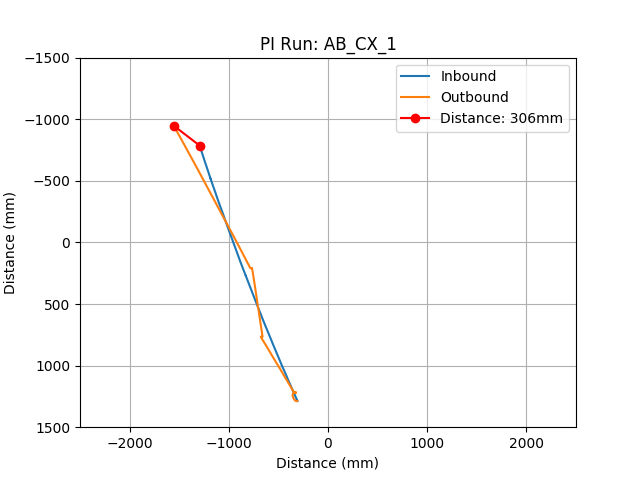
\includegraphics[width=0.8\textwidth]{AB_CX_1}
  \caption{\label{fig:abcx1} PI test AB\textunderscore
    CX\textunderscore 1}
\end{figure}

\begin{figure}[h!]
  \centering
  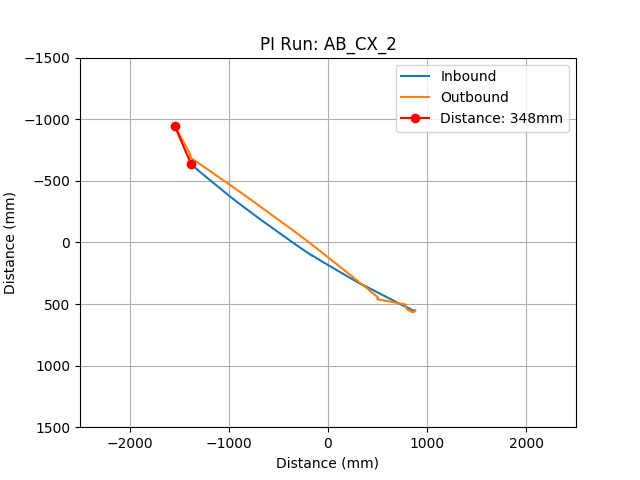
\includegraphics[width=0.8\textwidth]{AB_CX_2}
  \caption{\label{fig:abcx2}PI test AB\textunderscore
    CX\textunderscore 2}
\end{figure}

\begin{figure}[h!]
  \centering
  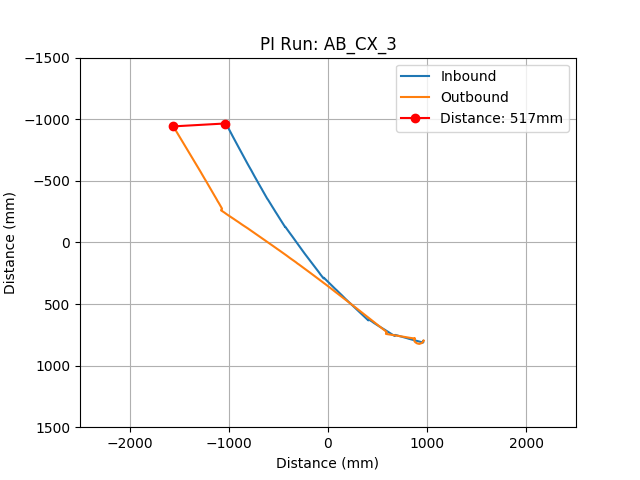
\includegraphics[width=0.8\textwidth]{AB_CX_3}
  \caption{\label{fig:abcx3}PI test AB\textunderscore
    CX\textunderscore 3}
\end{figure}

\begin{figure}[h!]
  \centering
  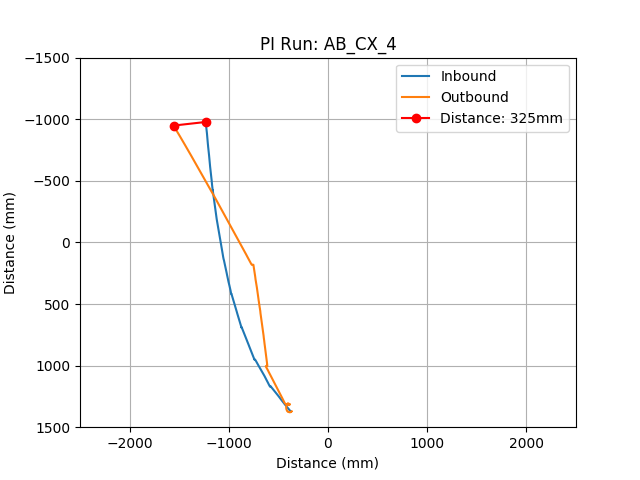
\includegraphics[width=0.8\textwidth]{AB_CX_4}
  \caption{\label{fig:abcx4}PI test AB\textunderscore
    CX\textunderscore 4}
\end{figure}

\begin{figure}[h!]
  \centering
  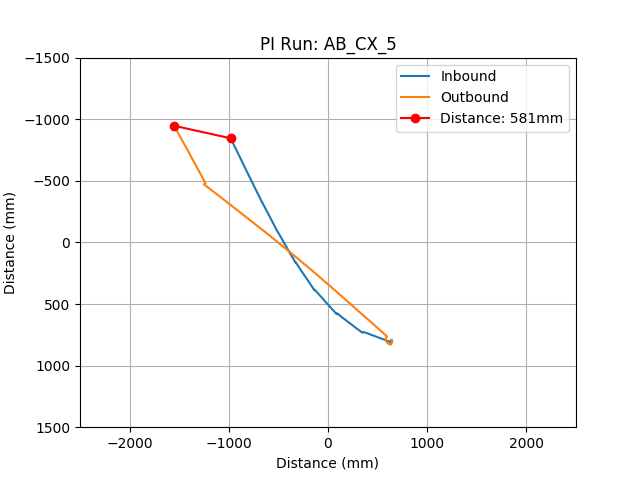
\includegraphics[width=0.8\textwidth]{AB_CX_5}
  \caption{\label{fig:abcx5} PI test AB\textunderscore
    CX\textunderscore 5}
\end{figure}

\begin{figure}[h!]
  \centering
  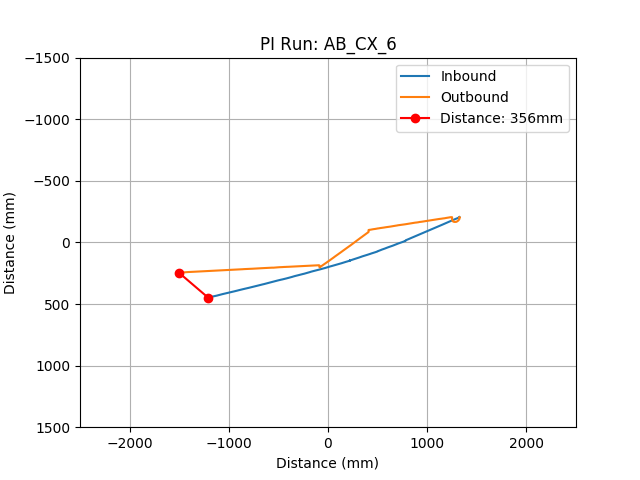
\includegraphics[width=0.8\textwidth]{AB_CX_6}
  \caption{\label{fig:abcx6} PI test AB\textunderscore
    CX\textunderscore 6}
\end{figure}

\begin{figure}[h!]
  \centering
  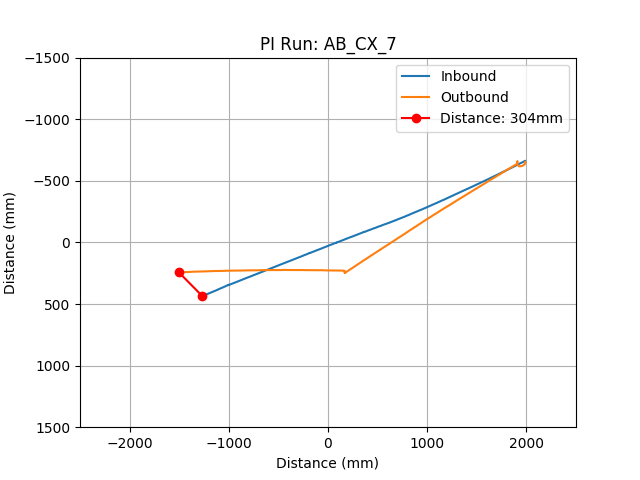
\includegraphics[width=0.8\textwidth]{AB_CX_7}
  \caption{\label{fig:abcx7} PI test AB\textunderscore
    CX\textunderscore 7}
\end{figure}

\begin{figure}[h!]
  \centering
  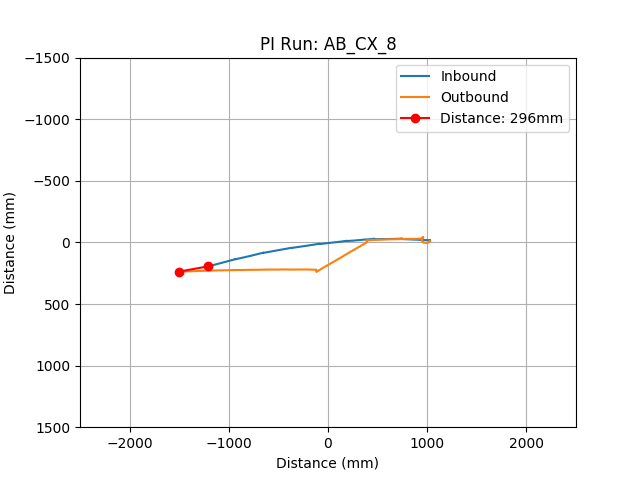
\includegraphics[width=0.8\textwidth]{AB_CX_8}
  \caption{\label{fig:abcx8} PI test AB\textunderscore
    CX\textunderscore 8}
\end{figure}

\begin{figure}[h!]
  \centering
  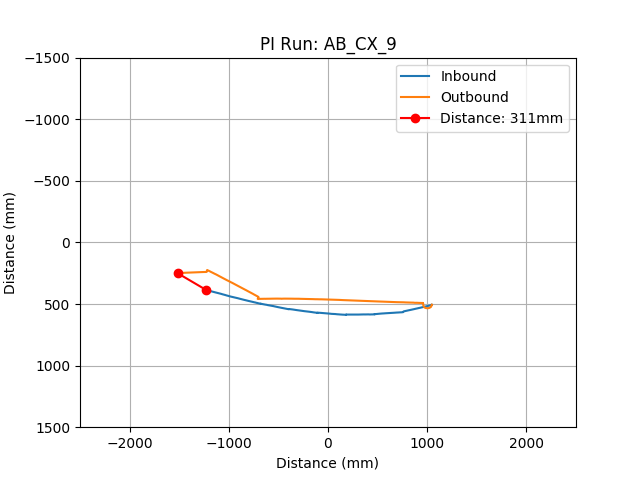
\includegraphics[width=0.8\textwidth]{AB_CX_9}
  \caption{\label{fig:abcx9} PI test AB\textunderscore
    CX\textunderscore 9}
\end{figure}

\begin{figure}[h!]
  \centering
  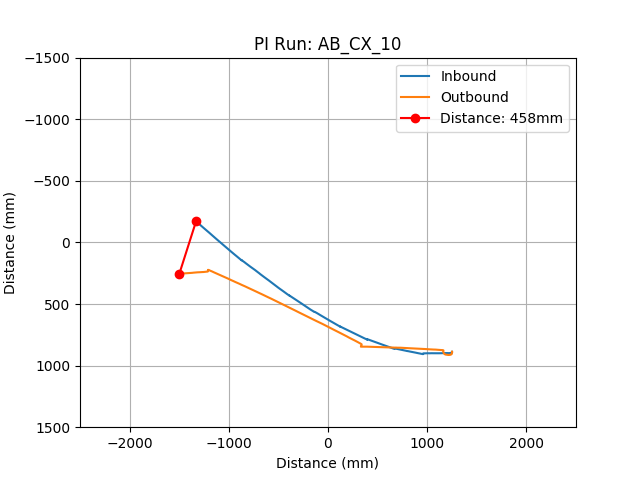
\includegraphics[width=0.8\textwidth]{AB_CX_10}
  \caption{\label{fig:abcx10} PI test AB\textunderscore
    CX\textunderscore 10}
\end{figure}
\end{document}

